\documentclass[a4paper,11pt]{book}
\newcommand{\Origin}{/home/fossee/Desktop/desk-new/cfd-openfoam}

\usepackage{color}
\usepackage{layouts}
\usepackage{cclicenses}
\usepackage{morefloats}
\usepackage{paralist}
\usepackage{chngcntr}
\usepackage{layouts}
\usepackage{fancyhdr}
\pagestyle{headings}
\usepackage{amsmath,graphicx,makeidx}
\usepackage{fancybox,url}
\usepackage{cite}
%\usepackage{appendix}
\counterwithout{footnote}{chapter}
\usepackage{subfig}
\usepackage{listings}
\usepackage{varioref} % for \vref commands
%\usepackage{hyperref}
\usepackage{array}

\newcommand{\redcolor}[1]{\color{red}#1\color{black}}
\newcommand{\codclr}{10pt}
\newcommand{\scilab}{Scilab}
\newcommand{\arduino}{Arduino Uno}
\newcommand{\ie}{\emph{i.e.},}

\newcommand{\ourname}[1]{\\ [1.5mm] \noindent{\bf #1}}
% Shroff book size
%\textheight 7.75in
\textheight 7.5in
\textwidth 5.5in
\evensidemargin 0.625in
\oddsidemargin 0.625in

\newcommand{\Home}{/home/fossee/Desktop/cfd-openfoam}

\newcommand{\tnfig}{0.3\linewidth}
\newcommand{\smfig}{0.45\linewidth}%0.42
\newcommand{\smfigp}{0.49\linewidth}%0.42
\newcommand{\lgfig}{0.65\linewidth}%0.65
\newcommand{\hgfig}{0.9\linewidth}

\renewcommand\bibname{References}

\newcommand{\figref}[1]{Fig.~\ref{#1}}
\newcommand{\figrefp}[1]{Fig.~\vref{#1}}
\newcommand{\tabref}[1]{Table~\ref{#1}}
\newcommand{\tabrefp}[1]{Table~\vref{#1}}
\newcommand{\chapref}[1]{Chapter~\ref{#1}}
\newcommand{\secref}[1]{Sec.~\ref{#1}}
\newcommand{\sciref}[1]{Scilab~Code~\ref{#1}}
\newcommand{\ardref}[1]{Arduino~Code~\ref{#1}}
\newcommand{\mypageref}[1]{Page~\pageref{#1}}
\newcommand{\fnref}[1]{Footnote~\ref{#1}}
\renewcommand{\topfraction}{1}
\renewcommand{\bottomfraction}{1}
\renewcommand{\textfraction}{0}
\renewcommand{\floatpagefraction}{1}
% \bibliographystyle{./IEEEtran}
\bibliographystyle{unsrt}

\hyphenation{Ashu-tosh pr-ess}

\makeindex
\begin{document}
\pagestyle{plain}
\pagestyle{empty}
\frontmatter
\thispagestyle{empty}
%\input{suppl/dedicate}
\pagestyle{headings}
\tableofcontents
\listoffigures
\listoftables
%\listofard
%\listofcode
%\thispagestyle{empty}
\addtocontents{toc}{\protect\thispagestyle{empty}}
%\input{suppl/preface}
%\input{suppl/acr}

\mainmatter
\pagestyle{headings}
\renewcommand\chaptermark[1]{\markboth{\bf {\thechapter. #1}}{}}
\renewcommand\sectionmark[1]{\markright{\bf {\thesection. #1}}}

%\input{texfiles/microcontintro.tex}
%\input{texfiles/sciaurint.tex}
%\input{suppl/intro.tex}
%\input{CHAPTERS/chap1/chapter1.tex} %rahul  
%\input{CHAPTERS/chap2/chapter2.tex} %suba
%\input{CHAPTERS/chap3/chapter3.tex} %suba
%\input{CHAPTERS/chap4/chapter4.tex} %suba
%\chapter{Downloading and Installing Salome}
\thispagestyle{empty}
\label{sec:chap5}
\newcommand{\LocCHfivefig}{\Origin/CHAPTERS/chap5/figures}

Salome is a Free and Open Source  CAD (Computer Aided Drawing), Meshing and Visualization Software for Numerical simulation. 
We can Create/modify, import/export (IGES, STEP, BREP), repair/clean CAD models and Mesh CAD models, edit mesh, check mesh quality, 
import/export mesh (MED, UNV, DAT, STL) using Salome. In this chapter we will learn how to download and intall Salome in any Operating system.

\section{Download Salome}

Open your browser and in the address bar type the url given below, \newline

\centering \textbf{www.salome-platform.org} \newline

\flushleft To Download Salome the user needs to create a account on the salome site. To do this on the left hand side of the salome screen website
scroll down to the bottom of the \textbf{Navigation} bar, Fig \ref{navi}, where you can see the new user option. Click on it and enter the required
personal details. \newline
\flushleft After you enter the details click on the register button at the bottom as shown in, Fig \ref{details}. Once done you will be directed 
to a screen showing that you have been registered. This also states thatv once you have done with registration you have to login to your email. Now 
open the mail sent by Salome and click on the link shown in Fig, \ref{link}. This link will direct you to a window where you need to set your password
for your Salome account. Enter the password and confirm it and press set my password button, Fig \ref{pass}. After this it will direct you to a window
which says your password has been set successfully. You may now login with your username and password. \newline

\flushleft In the Navigation bar click on Downloads after which you will be directed to a page which will show various bianaries for various Linux
distributions. You can choose according to your Operating System and 32/64 bit size. Since in this book we are working on a 64 bit platform we
will download Linux Debian 7 64-bits or Ubuntu 14.04 64-bits binary, Fig \ref{binary}. Click on it and Save the file. Since the file size is big it will take some time to download.
After this scroll down to Universal Binaries and click on the \textbf{Linux 64-bits} to download it. Note that 32-bit version of binaries are no
more supported for the latest version of Salome.

\begin{figure}[h]  
\centering
\includegraphics[scale=0.3]{\LocCHfivefig/navi.png}
\caption{Navigation Bar}
\label{navi}
\end{figure}

\begin{figure}[h]  
\centering
\includegraphics[scale=0.32]{\LocCHfivefig/details.png}
\caption{User Details}
\label{details}
\end{figure}

\begin{figure}[h]  
\centering
\includegraphics[scale=0.35]{\LocCHfivefig/link.png}
\caption{Salome Link}
\label{link}
\end{figure}

\begin{figure}[h]  
\centering
\includegraphics[scale=0.35]{\LocCHfivefig/pass.png}
\caption{Enter Password}
\label{pass}
\end{figure}

\begin{figure}[h]  
\centering
\includegraphics[scale=0.35]{\LocCHfivefig/binary.png}
\caption{Salome Linux Debain 7 64 bit binary}
\label{binary}
\end{figure}

\begin{figure}[h]  
\centering
\includegraphics[scale=0.45]{\LocCHfivefig/universal.png}
\caption{Universal Binaries}
\label{univ}
\end{figure}

\section{Installing Salome}

The downloaded files are saved in the Download folder. Open the Download folder in your system and check for both the tar file and a self-extracting file.
Copy these two files and in your home folder create a new folder by the name Salome and paste these two files inside it, Fig \ref{download}.


 %suba
%\input{CHAPTERS/chap6/chapter6.tex}
%\input{CHAPTERS/chap7/chapter7.tex}
%\input{CHAPTERS/chap8/chapter8.tex}
\chapter{Simulating Hagen Poiseuille flow}
\thispagestyle{empty}
\label{sec:chap9}
\newcommand{\LocCHninefig}{\Origin/CHAPTERS/chap9/figures}

\section{What is Hagen Poiseuille Law}

In nonideal Fluid Dynamics Hagen Poiseuille flow or Poiseuille law is a law which gives presure drop in a fluid flowing through a long cylindrical pipe.This law was experimentally derived independently by Gotthilf Heinrich Ludwig Hagen in 1839 and Jean Leonard Marie Poiseuille in 1838, and published by Poiseuille in 1840 and 1846. The assumptions of the equation are that the fluid is incompressible, Newtonian the flow is laminar through a pipe of constant circular cross-section that is substantially longer than its diameter and there is no acceleration of fluid in the pipe. For velocities and pipe diameters above a threshold, actual fluid flow is not laminar but turbulent, leading to larger pressure drops than calculated by the Hagen–Poiseuille equation.

\section{Problem Specification}

\begin{figure}[h]  
\centering
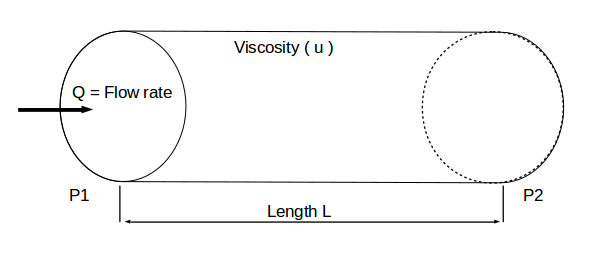
\includegraphics[scale=0.4]{\LocCHninefig/pipe.png}
\caption{Flow through a pipe}
\label{pipe}
\end{figure}

To simulate Hagen Poiseulle flow we consider a pipe of length 0.3m, diameter of 0.01m and fluid medium as water having a dynamic viscosity of $10^{-3}$. The pressure difference in along the pipe is taken as 20 Pascals.\newline

\flushleft Standard governing equations for Pressure drop in the pipe, Fig \ref{pipe} is given as follows, 

\begin{equation}
\nabla p = \frac{32 \mu_avg L }{D^2}
\end{equation}

\flushleft where $\nabla p$ is the pressure loss in the pipe, $\it{L}$ is the length of the pipe, $\mu$ is the dynamic viscosity, $\it{Q}$ is the volumetric flow rate, $\it{r}$ is the radius of the pipe.These parameters have been chosen to get a desired Reynolds number of 2080 which is under transient flow regime.\newline

\flushleft The maximum velocity in the pipe is given as,

\begin{equation}
U_max = 2*U_avg
\end{equation}

\flushleft Subsituting the values in equations above we get the value of $U_{max}$ around 0.416 $\frac{m}{s}$

\section{Geometry}

\begin{figure}[h]  
\centering
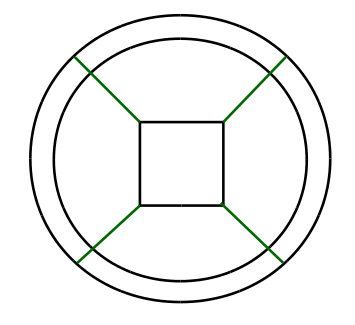
\includegraphics[scale=0.4]{\LocCHninefig/multi.png}
\caption{Multiblock grid}
\label{multi}
\end{figure}

\begin{figure}[h]  
\centering
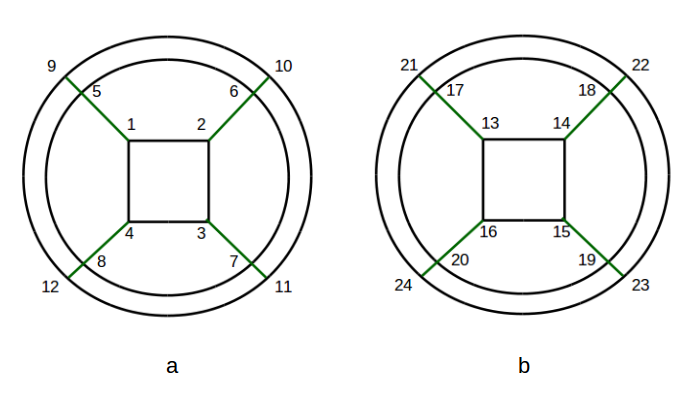
\includegraphics[scale=0.4]{\LocCHninefig/faces.png}
\caption{Back (a) and Front (b) faces for blockMesh}
\label{faces}
\end{figure}

For flow thorugh a pipe we will create a three dimensional pipe using blockMesh. We will use the multiblock meshing, \ref{multi}.This structure gives full control of the mesh grading, using edge meshing, with high-quality elements.Manual creation of multi-block structures can be usually more timeconsuming compared to unstructured meshes.It is seen that the mesh near the walls is required to be finer as compared to the center of the pipe as we can capture the wall shear stresses. In blockMesh we need to define the co-ordinates for each point for front and back faces as shown in the figure, \ref{faces}. For more details on creating a curved geometry in OpenFOAM, refer Chapter number 3. Since it's a 3D problem we will extrude the geometry along the Z direction. The meshing can be kept uniform with 20 cells along X and Y direction and 100 cells along Y direction.

\section{Solver}

Since the flow is still incompressible, viscous and laminar we will choose the solvers from incompressible flow category. We will choose the \textit{icoFoam} solver to solve this problem. \newline

\flushleft Create a folder inside the icoFoam solver directory and name it as pipe. Copy the 0, constant and system folders from the cavity case and paste it inside the newly created pipe folder. 

\subsection{constant}
To start with , make changes inside the blockMeshDict file located inside the polyMesh folder in constant. Edit the blockMeshDict file according to chapter number 3. 
After creating the faces using vertices, we now need to provide boundary names to the faces. This is required since so that we can Identify the different parts of the geometry during visualization and also use appropriate boundary coditions. In this case we have and Inlet, Outlet and walls as the boudnary condition. 

\subsection*{transportProperties}

The \textit{transportPropertis} file can be found inside the constant folder. We set the transport property of the fluid , in this case water and the dynamic visocity of water $\mu$ is taken as $1e^-6$ $\frac{m^2}{s}$
 
\subsection{0 (zero)}
Here we need to provide Initial boundary condition for the pipe. The \textit{0} folder contains files for \textit{pressure} and \textit{Velocity}. Appropriate boundary conditions are provided to solve the case.

\subsection*{p}

At Inlet we provide \textit{fixedValue} since we know the constant value at boundary which is 20 Pa. \newline
\flushleft The outlet is also given as \textit{fixedValue} boudnary condition since it is exposed to the atmosphere and taken as 0 Pa.\newline 
\flushleft The walls are given \textit{zeroGradient} boundary condition as the gradient of Pressure ($\nabla p$) is taken as 0. \newline
The dimension in the folder are given in terms of Kinematic pressure i.e dividing pressure with density and given a unit of $\frac{m^2}{s^2}$.

\subsection*{U}

Inlet boundary condition used for this case we will be \textit{pressureInletVelocity} boundary conditon. It is used when p is known at inlet, U is evaluated from the flux, normal to the patch. The value at inlet for u,v and w components of velocity can be kept as 0.  \newline
\flushleft Outlet boundary condition is taken as \textit{zeroGradient} as the gradient normal to the face is taken as zero. \newline
\flushleft Walls are given a no slip boundary condition and is given a \textit{zeroGradient} boundary condition with u,v and w components of velocity kept as 0.

\subsection{system}

The \textit{fvSchemes} and \textit{fvSolution} files can be kept default. We will change the time setting for our case. As this is a transient case, we keep the endTime of the solution as 20 sec with a time step ($\nabla t$) of $10^{-3}$. We need to make changes in other part of the file. \newline

\flushleft Once these settings are made we are now ready to run the case. Open a Terminal window and type in the path for the pipe folder in the icoFoam case directory of OpenFOAM. After this execute the commands as given below,

\begin{itemize}
\item blockMesh - This will generate the geometry and also mesh according to the mesh grading provided in the file. 
\item checkMesh - This command will check the validity of a mesh i.e Mesh quality, Skewness, number of cells , etc.
\item icoFoam - Run the solver to complete the simulation. The iterations running will be seen in the terminal window.
\end{itemize}

\section{Vizualization}

\begin{figure}[h]  
\centering
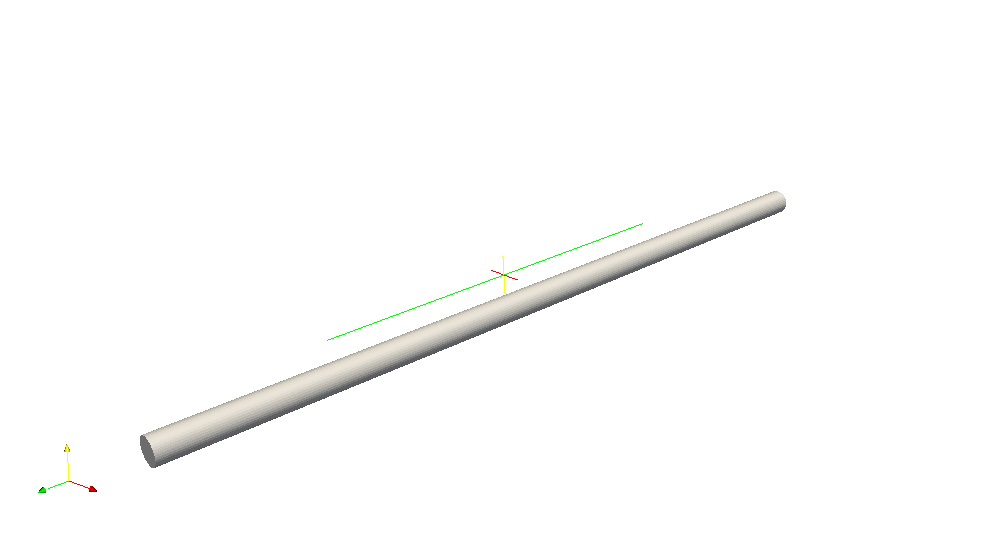
\includegraphics[scale=0.35]{\LocCHninefig/pipe1.png}
\caption{Pipe geometry as seen in Paraview}
\label{pipe_geom}
\end{figure}

\begin{figure}[h]  
\centering
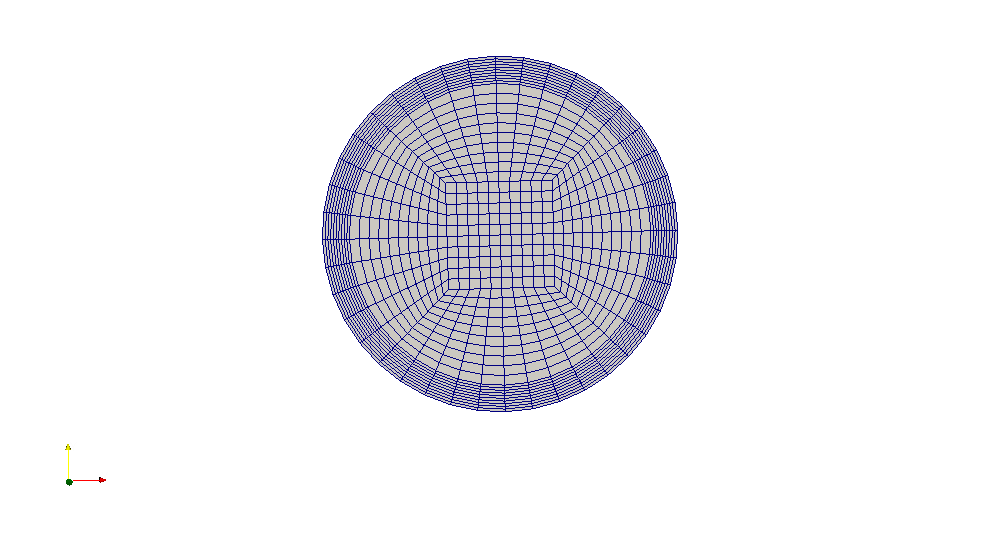
\includegraphics[scale=0.35]{\LocCHninefig/pipe2.png}
\caption{Multiblock mesh}
\label{pipe_mesh}
\end{figure}

\begin{figure}[h]  
\centering
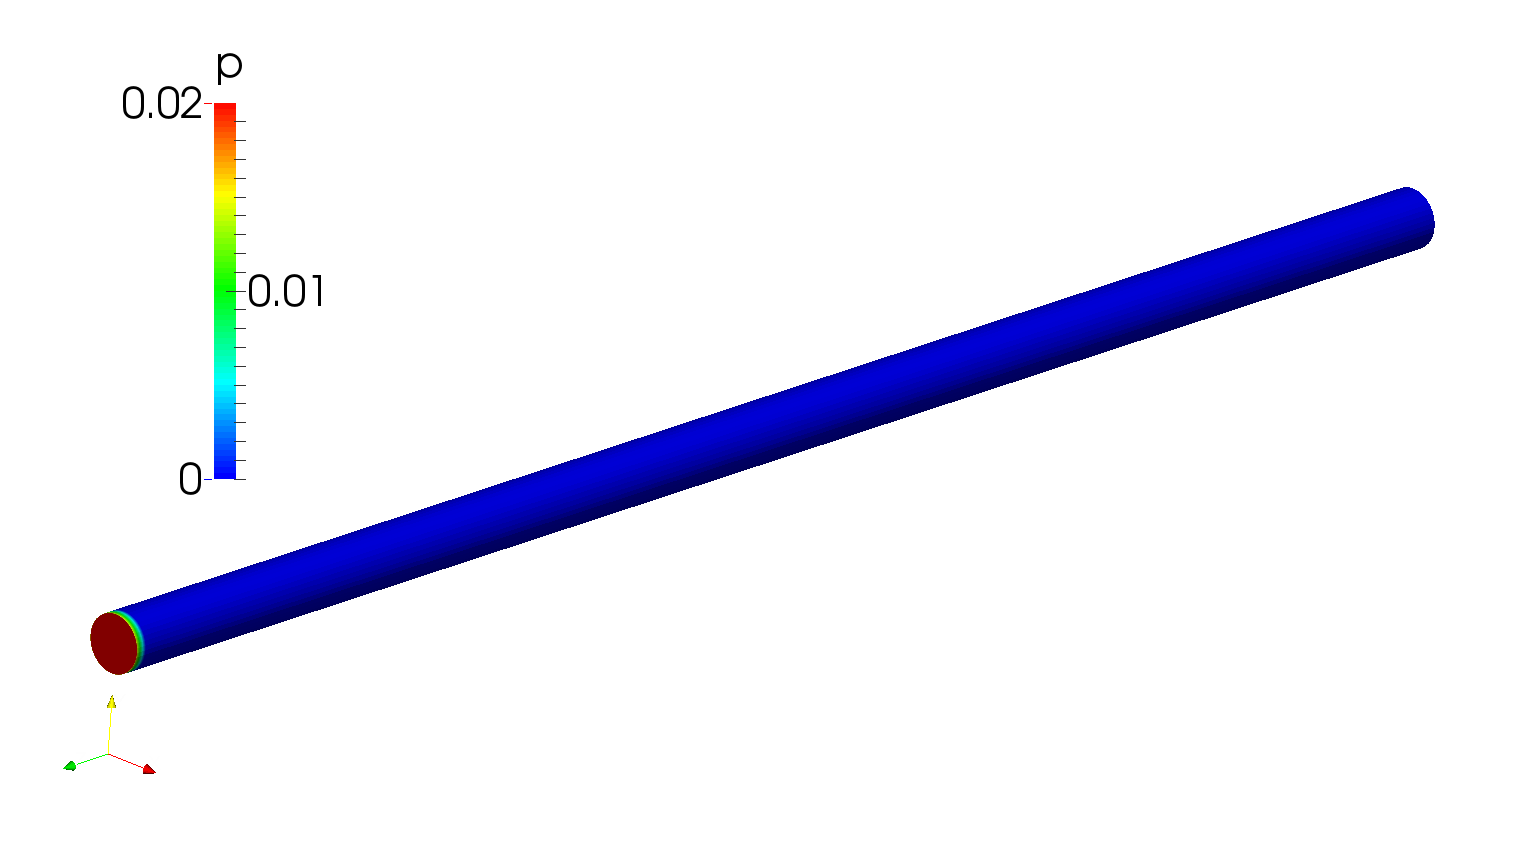
\includegraphics[scale=0.25]{\LocCHninefig/pressure.png}
\caption{Presure on inlet face at time, t = 0 sec}
\label{pipe_pressure}
\end{figure}

\begin{figure}[h]  
\centering
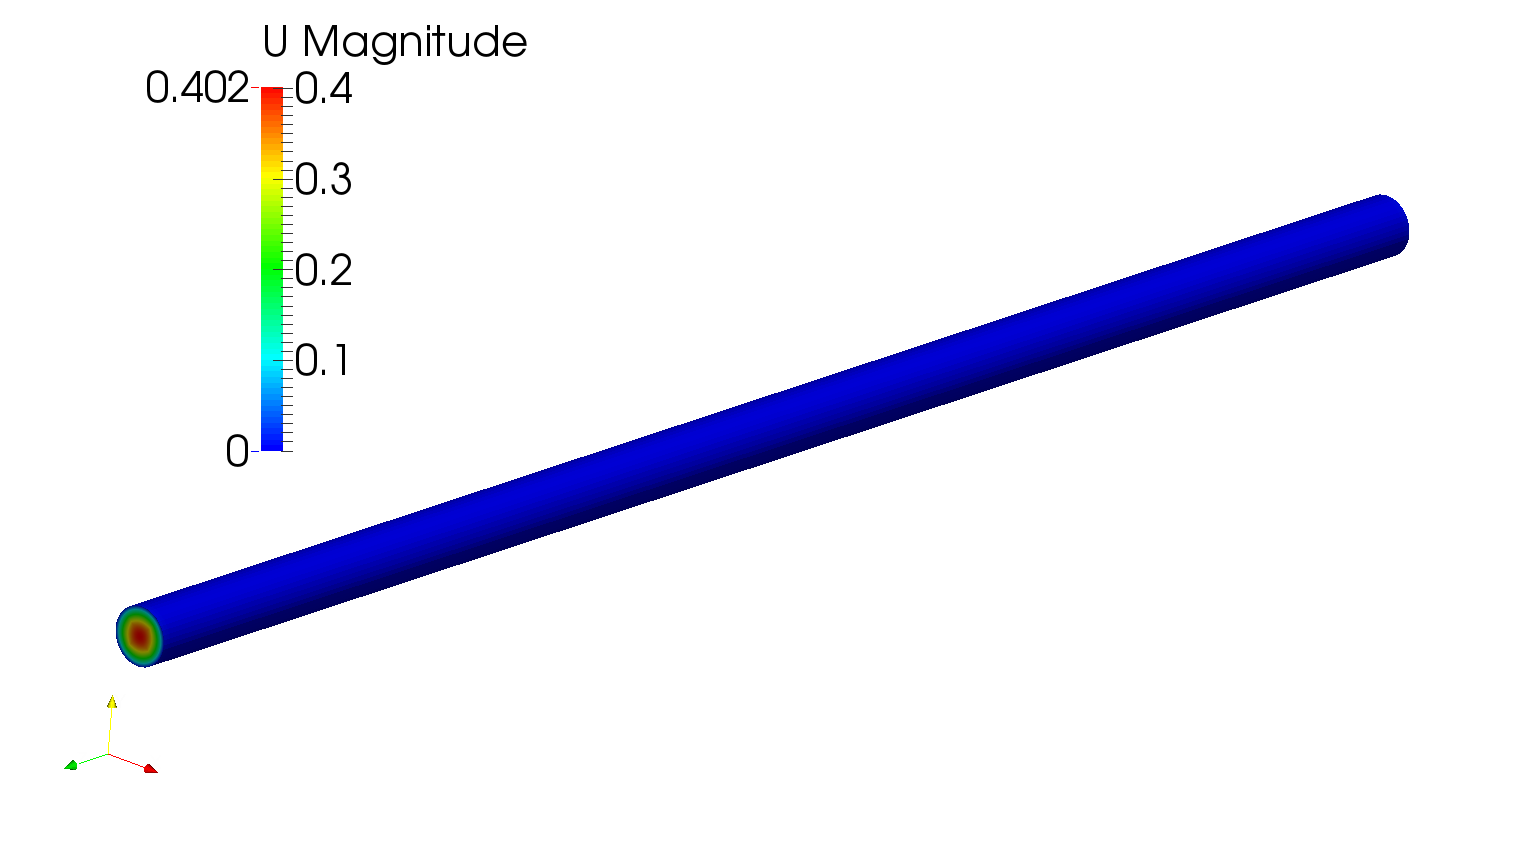
\includegraphics[scale=0.25]{\LocCHninefig/pipe_velocity.png}
\caption{Velocity in the pipe at time , t = 19 sec}
\label{pipe_velocity}
\end{figure}

\begin{figure}[h]  
\centering
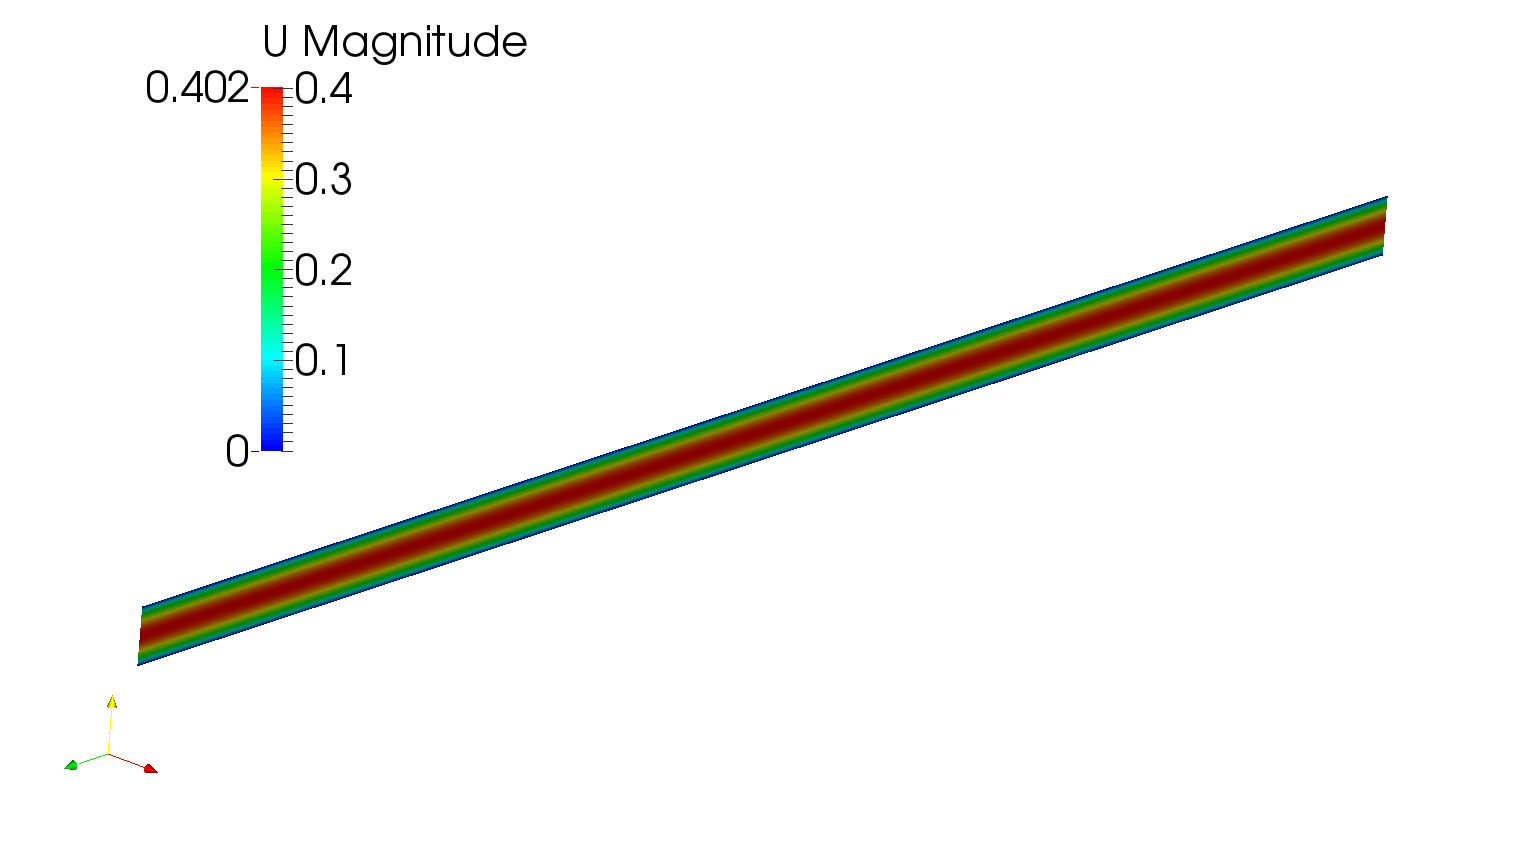
\includegraphics[scale=0.25]{\LocCHninefig/pipe_slice.png}
\caption{Cut section of the pipe showing velocity contour}
\label{pipe_slice}
\end{figure}

\begin{figure}[h]  
\centering
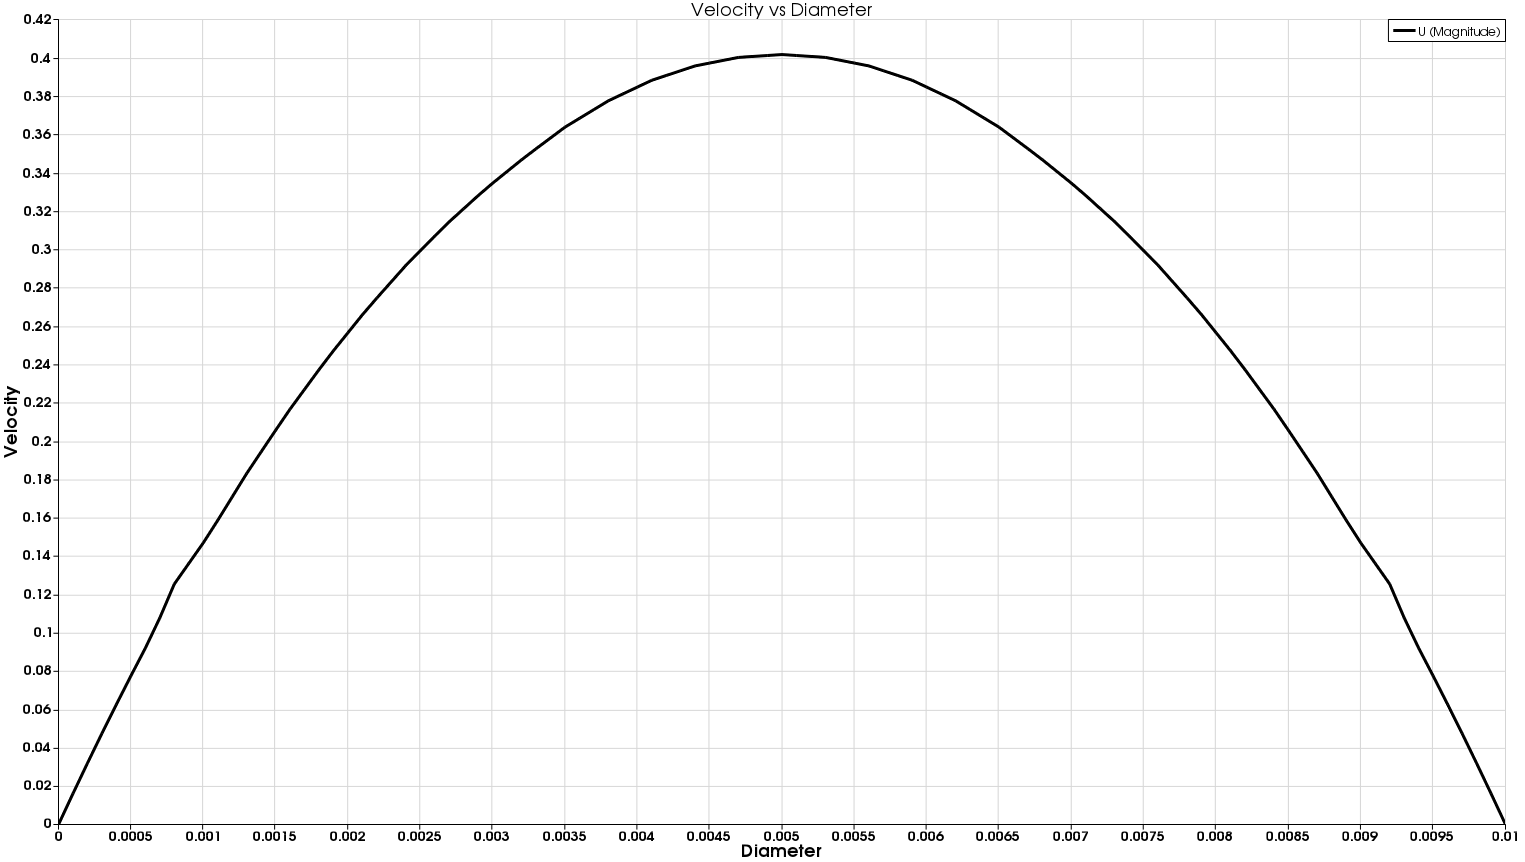
\includegraphics[scale=0.25]{\LocCHninefig/velocity.png}
\caption{Parabolic velocity profile for fully developed flow in the pipe}
\label{pipe_parabolic}
\end{figure}

To visualize the results type \textit{paraFoam} in the terminal and press enter. Click on the Apply button on the left hand Object Inspector menu. This opens up the pipe geometry as seen in Figure \ref{pipe_geom}. Since we have generated a multiblock mesh for this case, to view the same click on the drop down menu below VCR button and change from surface option to Surface with edges. The mesh can now be seen as having a coarse mesh near the center and fine mesh near the wall, Figure \ref{pipe_mesh}.To plot pressure and velocity contours for the pipe, first in the drop down menu change Solid Color to p (pressure). We can see the pressure at inlet of the pipe at time , t = 0 sec, Figure \ref{pipe_pressure}. Click on the play button on the top VCR menu and wait till it reaches the end time of 19 sec. In the drop down menu now change from p (pressure) to U (Velocity) which shows the velocity of the fluid at 19 sec in the color legend as 0.401 $\frac{m}{s}$ as calculated from analytical results. To display the cross section of the pipe on the Top menu in paraview go to \textit{Filter / Alphabetical / Slice }, select as slice along Y axis to get a cut section of the pipe, Figure  \ref{pipe_slice}. The flow developes a parabolic profile once it reaches a sufficient development length. To plot the velocity profile for the flow, go to \textit{Filters / Alphabetical / Plot over Line} and select Y axis and click on Apply. A new window will open showing plots of velocity, pressure. Now scroll down the property pannel and select p ( pressure ) check box. We can see the parabolic velocity profile as seen in the Figure \ref{pipe_parabolic}.

\section{Assignment}

Create a pipe having a diameter of 0.02 m and length of 0.4 m. Pressure at the inlet of the pipe is 100 Pascals and atmospheric at the outlet. Calculate the reynolds number for this flow for a fluid having viscosity of $10^{-6}$ $\frac{m^2}{s}$Carry out simulation for a course grid and a fine grid. Compare both the solution obtained in both the cases. 
\chapter{Downloading and Installing Salome}
\thispagestyle{empty}
\label{sec:chap10}
\newcommand{\LocCHtenfig}{\Origin/CHAPTERS/chap10/figures}

Salome is a Free and Open Source  CAD (Computer Aided Drawing), Meshing and Visualization Software for Numerical simulation. 
We can Create/modify, import/export (IGES, STEP, BREP), repair/clean CAD models and Mesh CAD models, edit mesh, check mesh quality, 
import/export mesh (MED, UNV, DAT, STL) using Salome. In this chapter we will learn how to download and intall Salome in any Operating system.

\section{Download Salome}

Open your browser and in the address bar type the url given below, \newline

\centering \textbf{www.salome-platform.org} \newline

\flushleft To Download Salome the user needs to create a account on the salome site. To do this on the left hand side of the salome screen website
scroll down to the bottom of the \textbf{Navigation} bar, Fig \ref{navi}, where you can see the new user option. Click on it and enter the required
personal details. \newline
\flushleft After you enter the details click on the register button at the bottom as shown in, Fig \ref{details}. Once done you will be directed 
to a screen showing that you have been registered. This also states thatv once you have done with registration you have to login to your email. Now 
open the mail sent by Salome and click on the link shown in Fig, \ref{link}. This link will direct you to a window where you need to set your password
for your Salome account. Enter the password and confirm it and press set my password button, Fig \ref{pass}. After this it will direct you to a window
which says your password has been set successfully. You may now login with your username and password. \newline

\flushleft In the Navigation bar click on Downloads after which you will be directed to a page which will show various bianaries for various Linux
distributions. You can choose according to your Operating System and 32/64 bit size. Since in this book we are working on a 64 bit platform we
will download Linux Debian 7 64-bits or Ubuntu 14.04 64-bits binary, Fig \ref{binary}. Click on it and Save the file. Since the file size is big it will take some time to download.
After this scroll down to Universal Binaries and click on the \textbf{Linux 64-bits} to download it. Note that 32-bit version of binaries are no
more supported for the latest version of Salome.

\begin{figure}[h]  
\centering
\includegraphics[scale=0.3]{\LocCHtenfig/navi.png}
\caption{Navigation Bar}
\label{navi}
\end{figure}

\begin{figure}[h]  
\centering
\includegraphics[scale=0.32]{\LocCHtenfig/details.png}
\caption{User Details}
\label{details}
\end{figure}

\begin{figure}[h]  
\centering
\includegraphics[scale=0.35]{\LocCHtenfig/link.png}
\caption{Salome Link}
\label{link}
\end{figure}

\begin{figure}[h]  
\centering
\includegraphics[scale=0.35]{\LocCHtenfig/pass.png}
\caption{Enter Password}
\label{pass}
\end{figure}

\begin{figure}[h]  
\centering
\includegraphics[scale=0.35]{\LocCHtenfig/binary.png}
\caption{Salome Linux Debain 7 64 bit binary}
\label{binary}
\end{figure}

\begin{figure}[h]  
\centering
\includegraphics[scale=0.45]{\LocCHtenfig/universal.png}
\caption{Universal Binaries}
\label{univ}
\end{figure}

\section{Installing Salome}

The downloaded files are saved in the Download folder. Open the Download folder in your system and check for both the tar file and a self-extracting file.
Copy these two files and in your home folder create a new folder by the name Salome and paste these two files inside it. Extract the tar file files inside Salome folder. Open the command terminal and type the path for the Salome folder that we just created. Inside this type the path for the InstallWizard $\_$7$\_$Debian$\_$7.0$\_$64bits. Type ls in the terminal to view the content inside the directory. Now to install Salome we will type :
./runInstall -b and press enter. The user will be asked for selecting the platform. Press 1 to Select the Debian platform. Close the  terminal once this process is finished. Open a new command terminal and type ./S and press the tab key. Since Ubuntu is case sensitive it will recognize the initial letters and Open the required folder. Hit enter to execute the .run file. Press enter again to select the default path or you can provide a path of your choice. The user will again be interrupted for choosing the language for installation of Salome in French, type N and press enter. The installation process will begin and will take a while. Once this is done we will see Salome Icon on in the Desktop, we can double click on it to Open the software. Thus this brings us to the end of this chapter on Installation of Salome. 




 %rahul
\chapter{Creating and Meshing a curved pipe geometry in Salome for OpenFOAM}
\thispagestyle{empty}
\label{sec:chap11}
\newcommand{\LocCHelevenfig}{\Origin/CHAPTERS/chap11/figures}

This chapter deals with Creating a curved pipe geometry ( pipe bend ) using Salome and Meshing it.The curved pipe system is important in power plants and process industries. It is often important to predict flow field and temperature fields in the neighborhood of the mixing region in order to properly design the location of inlet pipes.

\section{Prerequisite}
The chapter assumes that the user has worked through the previous chapter on Salome Installation and has it running in his system

\section{Problem Description}

The problem to be considered is shown Schematically in Figure. The dimensions used here are in mm.We will use the bottom-up approach here. This approach means that you will first create some vertices, connect the vertices with edges and connect the edges. The only difference here is that wwe would be used a divided disc approach to create a face for the pipe which will be then extruded along the path to complete the 3D pipe.

\section{Procedure}

Start Salome by clicking the icon on your desktop. This will open up the Salome working window Figure, \ref{salome}. \newline

\begin{figure}[h]  
\centering
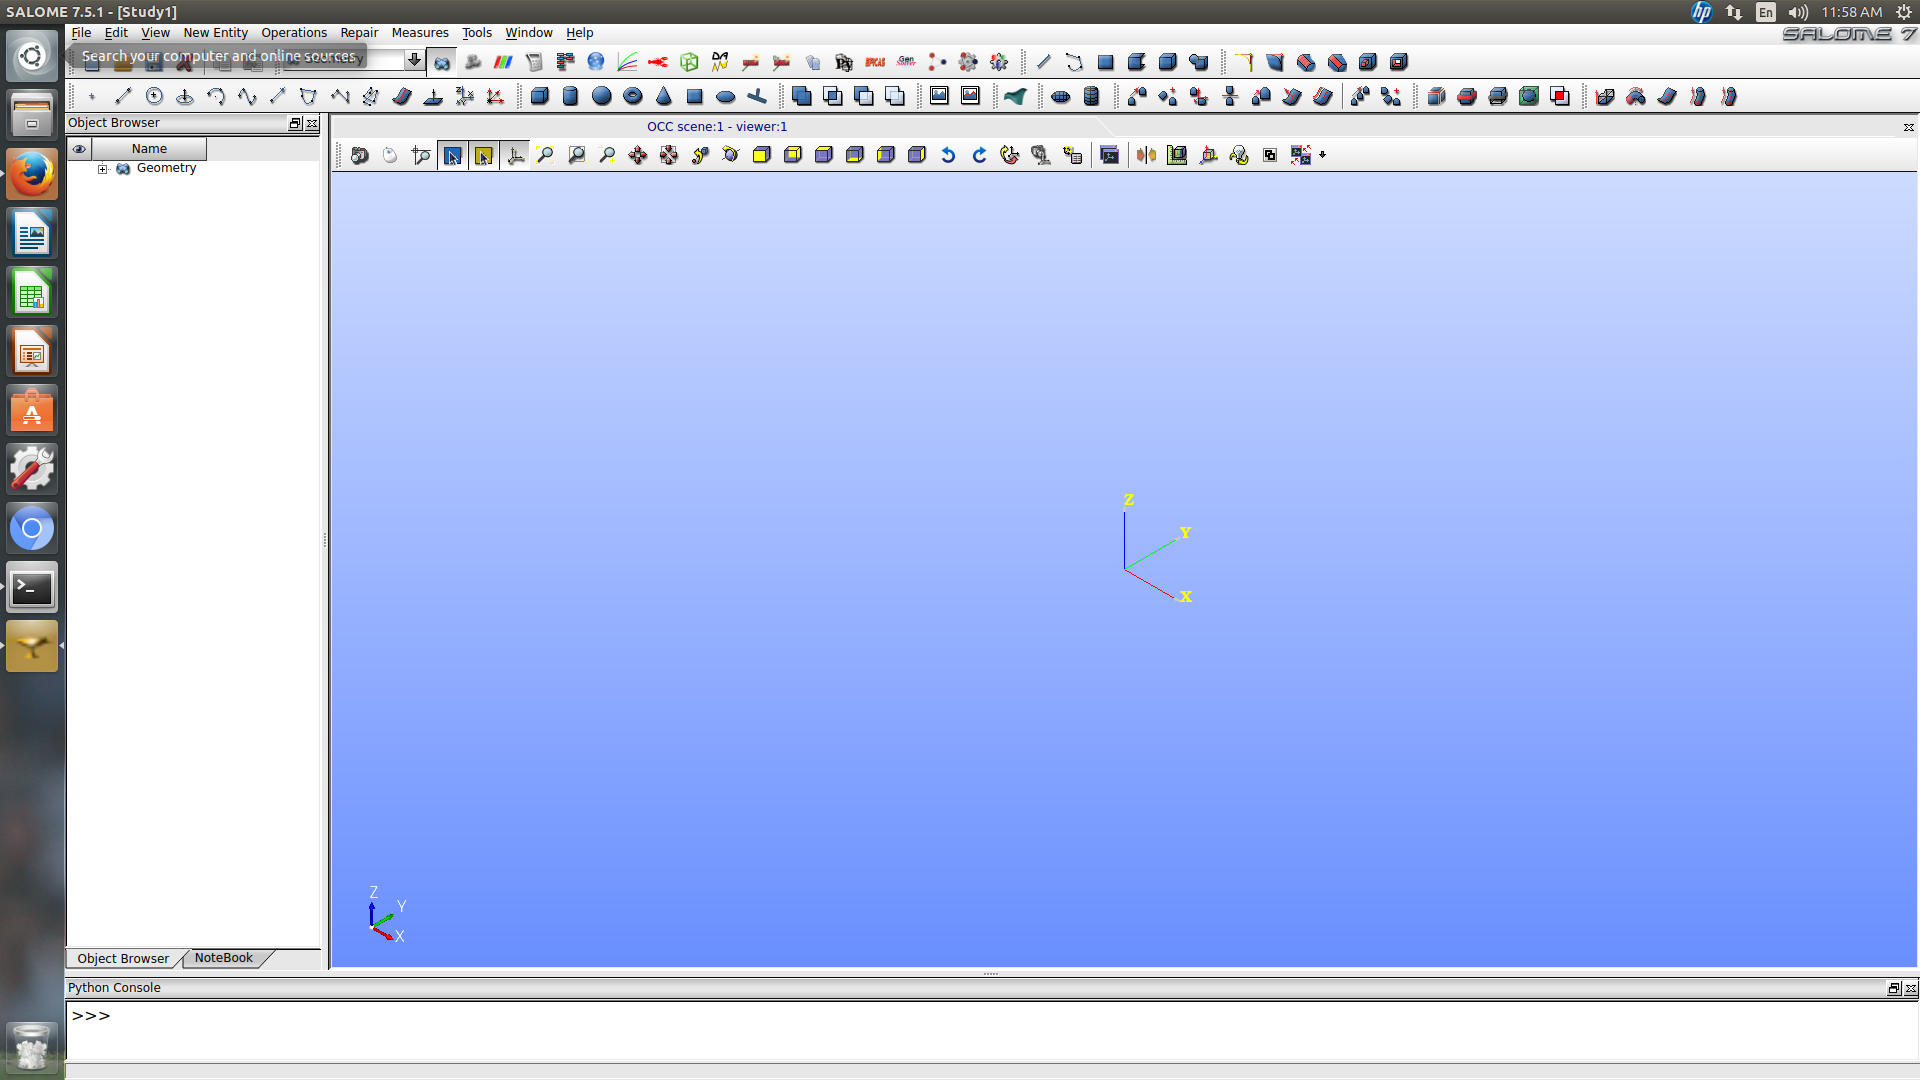
\includegraphics[scale=0.35]{\LocCHelevenfig/salome1.png}
\caption{Salome working window}
\label{salome}
\end{figure}

\subsection*{Active Module}

\begin{figure}[h]  
\centering
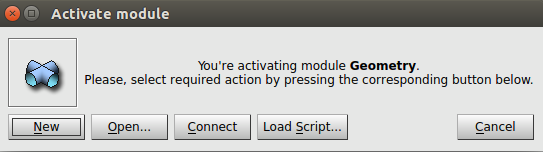
\includegraphics[scale=0.45]{\LocCHelevenfig/activate.png}
\caption{Activate module to open new file}
\label{activate}
\end{figure}

To create geometry we first need to select Geometry from the module drop down menu. We will open up a window which says Activate module,Figure. In this the user can Open a new window, Open an already created file , connect to different systems or Load an exsiting python script. Since we do not have an existing geometry we will create a new geometry here, so click on the New tab, Figure \ref{activate} . 

\subsection*{Geometry Properties}

\begin{figure}[h]  
\centering
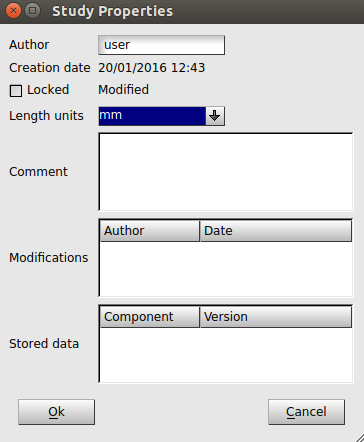
\includegraphics[scale=0.45]{\LocCHelevenfig/salome_prop.png}
\caption{Property table to set dimension}
\label{prop}
\end{figure}

After this on the top menu bar, click on File/Preference. This opens up the preference window where we can set the dimensions for our geometry, Figure \ref{prop}. Name of the Author can be the user. You can lock the dimensions for all your cases by clicking on the Locked buton below author. In the drop down menu besides Length, change it to mm. Other parts of the property panel can be kept default.

\subsection*{Geometry}

\begin{figure}[h]  
\centering
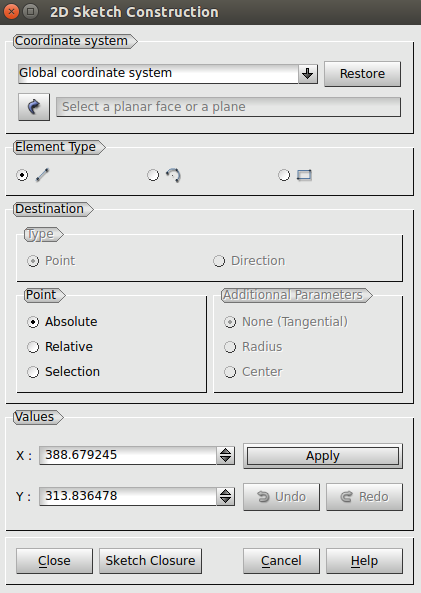
\includegraphics[scale=0.45]{\LocCHelevenfig/2dsketch.png}
\caption{2D Sketch construction window}
\label{point}
\end{figure}

To create geometry we will first create our base point. To do this launch the 2D Sketcher by clicking on the top menu \textit{New Entity/ Basic / 2D Sketch}. Enter the coordinates of the point of origin (0, 0) and click the Apply, Figure \ref{point}. Create the 1st Vertical segement using Line type element / Destination - Point/ Point - Absolute and enter the values (0, 30). We will now create an arc for our pipe bend, by Selecting the Element Type- Arc/ Destination - Direction/ Direction - Tangent and enter the values for Radius as -10 and Angle as 90 degree. The horizontal line can be drawn using Element type - Line / Destination - Direction / Direction - Tangent and enter the length for line as 30. Click on the close button. Do not click on the Sketch Closure button as this will join the starting point and the end point by a line.

\subsection*{DividedDisk}

\begin{figure}[h]  
\centering
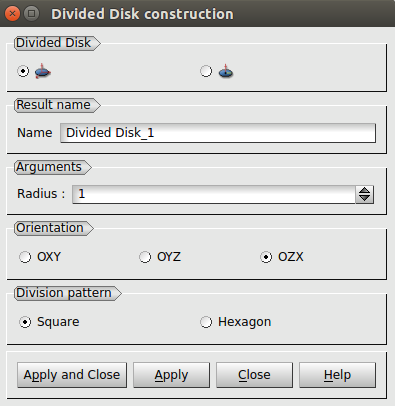
\includegraphics[scale=0.45]{\LocCHelevenfig/divideddisk.png}
\caption{Divided Disk Construction window}
\label{disk}
\end{figure}

We will now create a face for inlet of our pipe using Divided Disk object. It is a disk divided into blocks for easy hexahedral meshing. Two division patterns are available a Square pattern and a Hexagonal pattern. This can done by \textit{ New Entity/ Blocks / Divided Disk}. Divided Disk construction will open up, enter in this the Radius of the pipe as 1, orientation is the plane on which the disk will be built as OZX and the division pattern as square, Figure \ref{disk}. Click on Apply and Close.Final geometry will be as seen in the Figure \ref{disk1} 

\begin{figure}[h]  
\centering
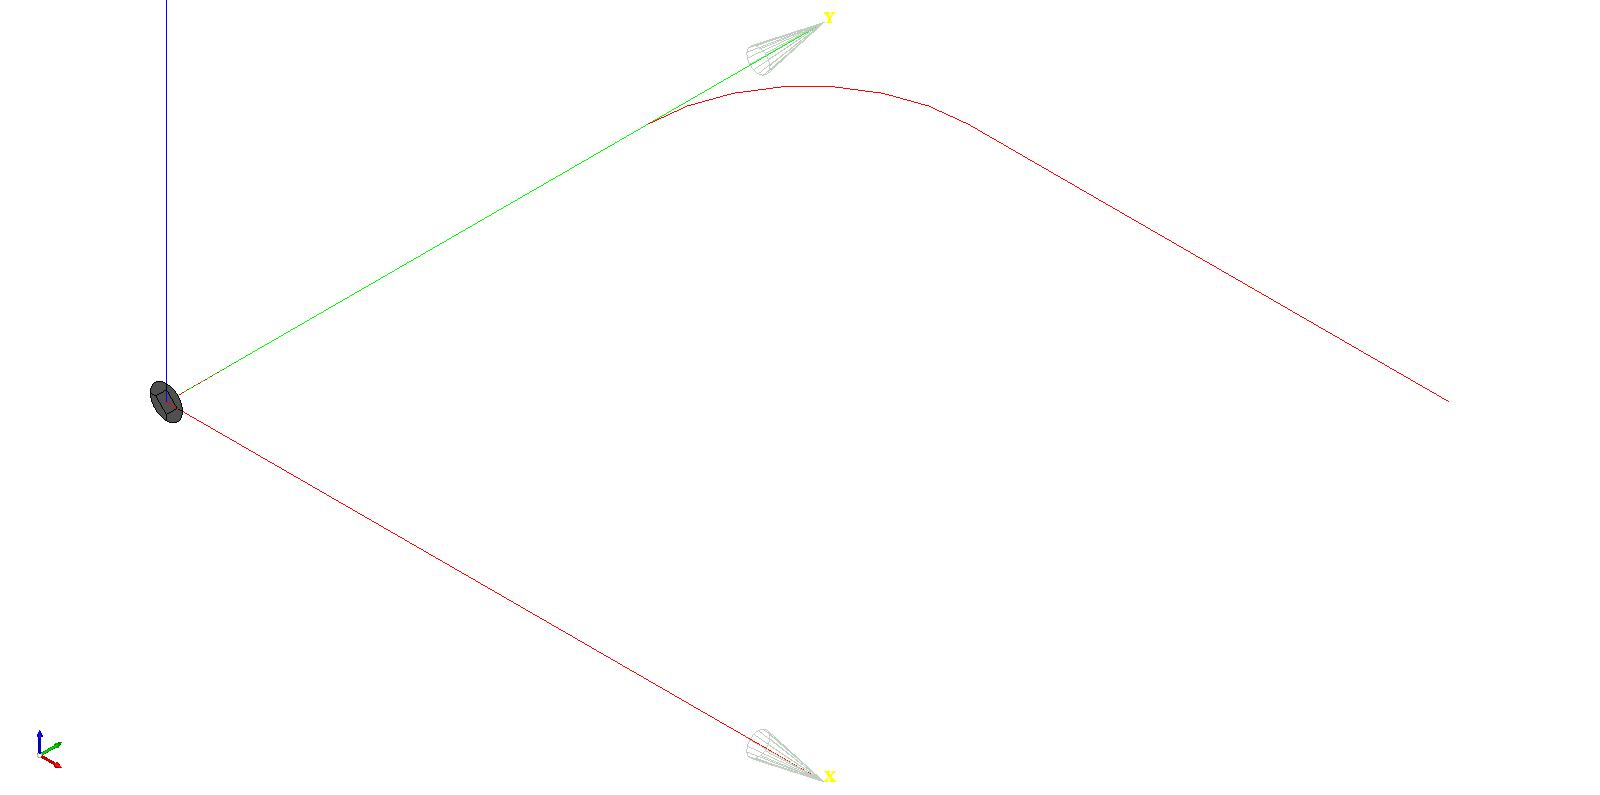
\includegraphics[scale=0.35]{\LocCHelevenfig/divideddisk1.jpg}
\caption{Inlet face using divided disk}
\label{disk1}
\end{figure}

\subsection*{Extruction}

\begin{figure}[h]  
\centering
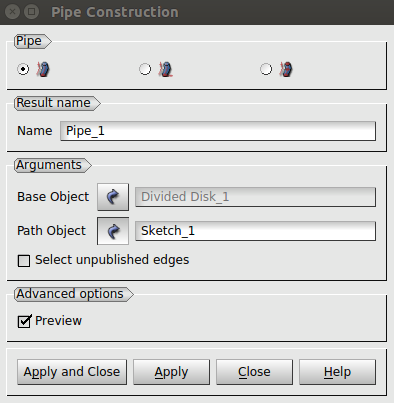
\includegraphics[scale=0.35]{\LocCHelevenfig/pipeconst.png}
\caption{Pipe Cnstruction window}
\label{pipeconst}
\end{figure}

\begin{figure}[h]  
\centering
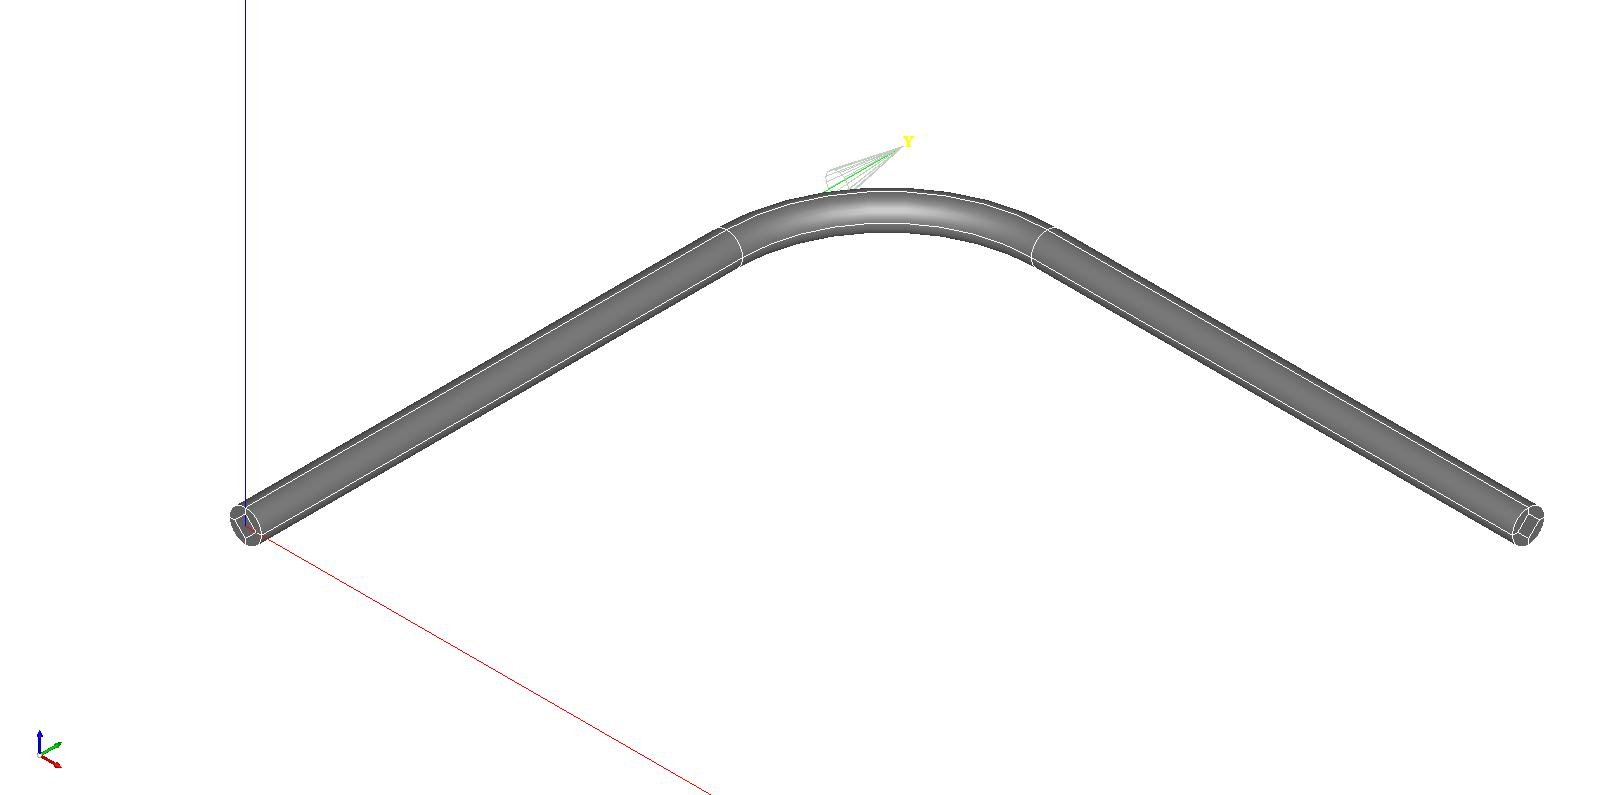
\includegraphics[scale=0.35]{\LocCHelevenfig/salome_pipe.jpg}
\caption{3D pipe bend}
\label{3dpipe}
\end{figure}

For construction of the 3D pipe we need to extrude the face created using divided disk along the curve generated earlier. Click on \textit{New Entity/ Generate / Extrude Along path}. In the Pipe constrution window name the pipe as Pipe-1, base object as Divided Disk-1 and the Patch Object as Sketch-1, Figure \ref{pipeconst}. Click Apply to close the window.3D bent pipe is now constructed as seen in the Figure \ref{3dpipe}.    

\subsection*{Explode}

\begin{figure}[h]  
\centering
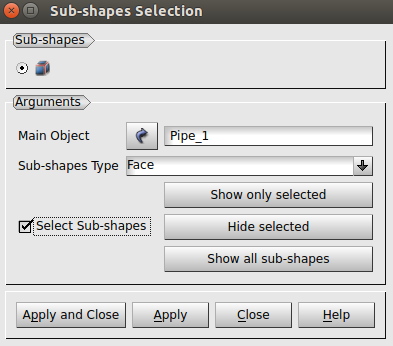
\includegraphics[scale=0.35]{\LocCHelevenfig/subshape.png}
\caption{Sub-Shape selection dialog box}
\label{subshape}
\end{figure}

\begin{figure}[h]  
\centering
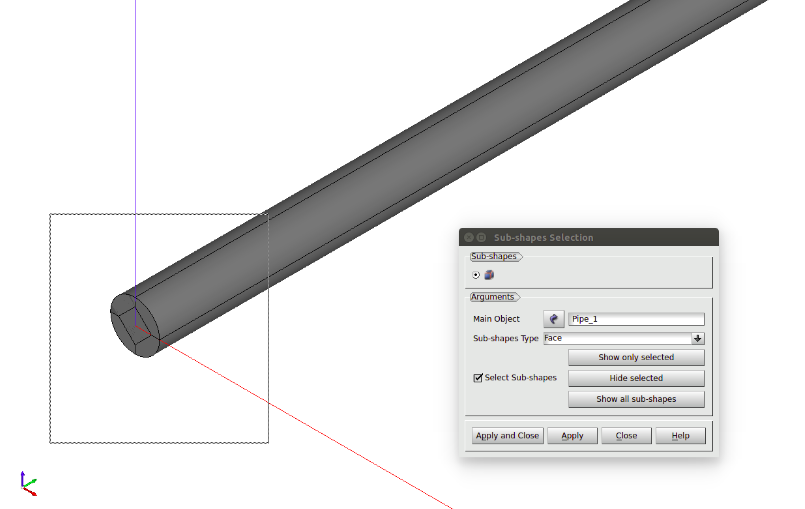
\includegraphics[scale=0.35]{\LocCHelevenfig/subshape_inlet.png}
\caption{Sub-Shape face selection for Inlet face}
\label{subshape_inlet}
\end{figure}

\begin{figure}[h]  
\centering
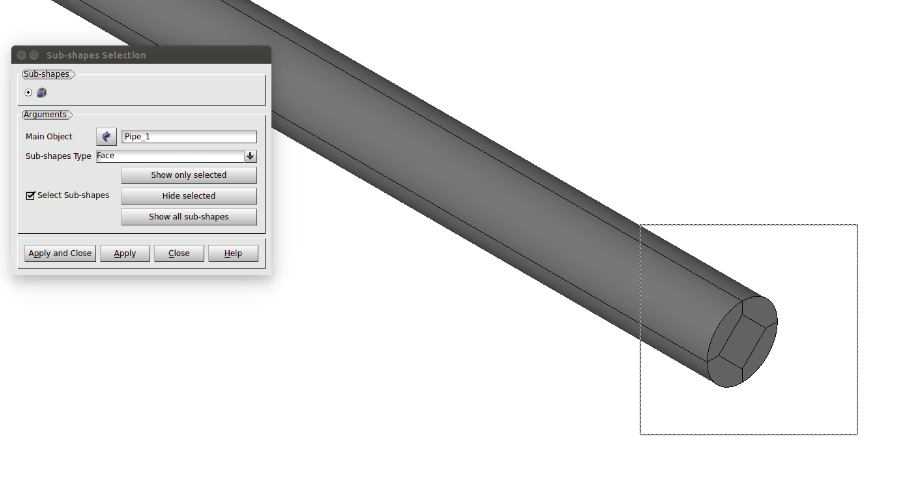
\includegraphics[scale=0.35]{\LocCHelevenfig/subshape2.png}
\caption{Sub-Shape face selection for Outlet face}
\label{subshape_outlet}
\end{figure}

To explode an object into sub-shapes in the Main menu slect \textit{New Entity / Explode}. This operation opens the sub shape selection dialog box. It is useful since we can extract the solid, face, edges, points needed to group. For our case , select the main object as Pipe-1, Sub-shape Type as Face. Also click on the Select Sub-Shape check box to select the required subshape, Figure \ref{subshape}. Now we will first select the inlet face first. To do this using the left click of the mouse drag your curser over the inlet face as seen in the Figure \ref{subshape_inlet}. The edges of the face would turn white. Now click on the Show only selected tab , to see the selected face and click Apply and Close.Repeat the procedure for outlet face as well.On the left hand side of the working window we can see the 10 faces under Object Tree structure. \newline

\begin{figure}[h]  
\centering
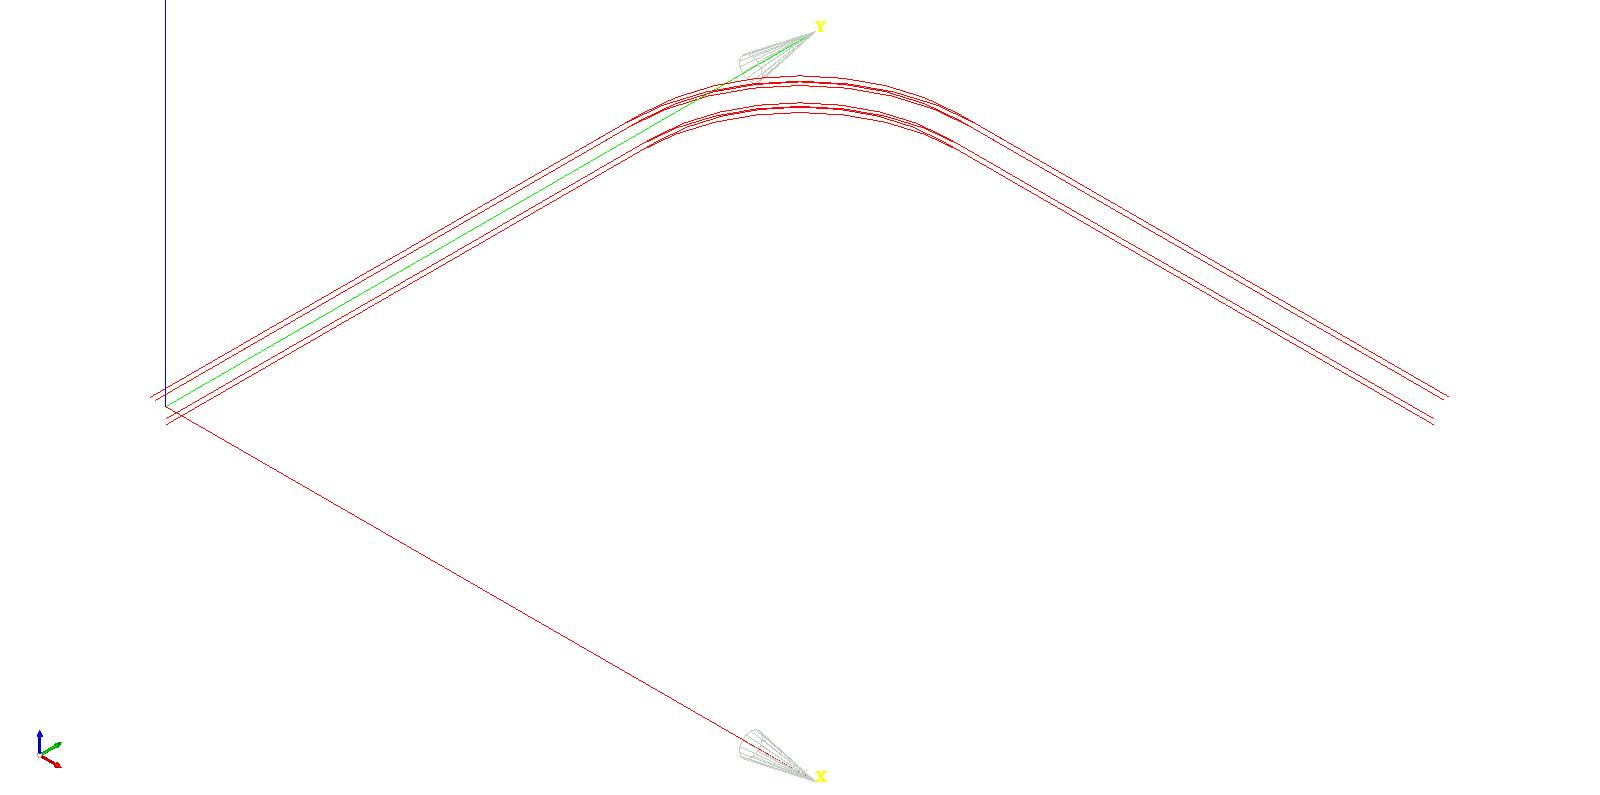
\includegraphics[scale=0.35]{\LocCHelevenfig/edges.jpg}
\caption{Exploded edges}
\label{edges}
\end{figure}

\flushleft We will also explode the edges along the flow direction. This is required since we need a finer mesh along the flow direction. Click on the \textit{New Entity / Explode} option. In the Sub-shape selection dialog box select the Main object as Pipe-1 and the Sub-shapes as Edges since we need to explode edges to group them. Select the Sub-shapes box and then Drag your right click mouse pointer over the inlet face and click on Hide Selected to hide the face as we want only the edges. Repeat this process for remaining faces. Finally drag the mouse pointer over edges as shown in the Figure \ref{edges} and click on Apply and Close. On the right hand side in Object browser tree we will see seperate 24 edges.

\subsection*{Groups}

\begin{figure}[h]  
\centering
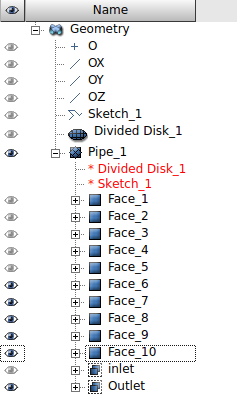
\includegraphics[scale=0.45]{\LocCHelevenfig/tree_salome.png}
\caption{Object browser tree}
\label{tree-salome}
\end{figure}

This operation allows creating groups on all selected shapes. Only the main shape of the geometry and Subshape needs to be selected. Click on \textit{New Entity/ Group / Create Group}. A Create Group window will pop-up. Under shape type select Face, name the group as Inlet, choose the main shape as Pipe-1. Select the first five faces (1-5) as subshape and Click on Add. Click Apply and Close to see the inlet group cerated in the Object tree browser. Repeat the same process for the outlet faces by selecting the faces (6-10) and name the group as Outlet, Figure \ref{tree-salome}. Now to group the edges along flow direction in Create Group dialog box select edges, Name the group as flow-direction, main shape as Pipe-1 and select the 24 edges exploded and Click on the Apply and Close button to create a group for flow-direction edges.This will help us in identifying the faces when we export the geometry for Simulation.

\section{Meshing Module}

\begin{figure}[h]  
\centering
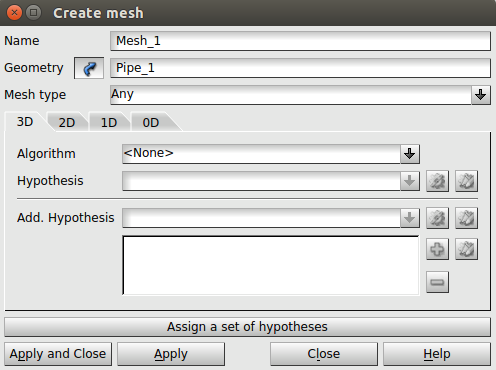
\includegraphics[scale=0.35]{\LocCHelevenfig/mesh.png}
\caption{Create mesh dialog box}
\label{edges}
\end{figure}

\begin{figure}[h]  
\centering
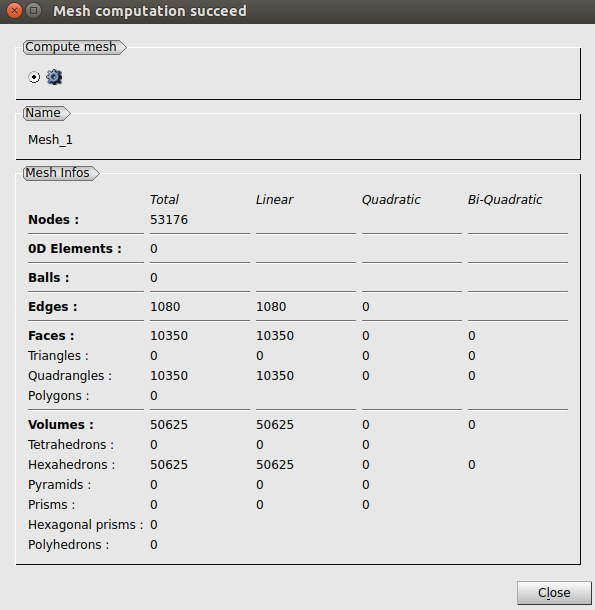
\includegraphics[scale=0.35]{\LocCHelevenfig/mesh_info.png}
\caption{Mesh information box}
\label{meshinfo}
\end{figure}

The goal of this module is to create meshes on the basis of geometrical models created or imported in the Geometry Module. It uses a set of meshing algoriths and their corresponding conditions (hypothesis) to compute meshes. Click on the Modules drop down Menu and change it from Geometry to Mesh. To mesh our geometry click on \textit{Mesh / Create Mesh}, this will open the Create Mesh dialog box, Figure . Name the mesh as Mesh-1, Select the geometry as Pipe-1 and click on the Assign a Set of hypotheses button to Select 3D: Automatic Hexahedralization. This will open up another dialog box , in this enter the Number of Segments as 15. Click OK to close this box and click on Apply and Close to close the create mesh box.Now in the Object browser tree rght click on Mesh-1 and selct Compute. This will mesh our geometry.A dialog box will appear at the end of Meshing providing the mesh information , Figure \ref{meshinfo}.\newline

\flushleft To save the Geometry, click on the File menu in the menu bar and click on Save As. Name the file as curved-geometry and the file format as .hdf ( a standard developed by Boeing and NASA in the aera of CFD ).

\section{Assignment}

As a practice assignment create a curved pipe having a radius of 1.5 mm and total length of 200 mm. Mesh the geometry and save it. 



\chapter{Exporting geometry from Salome to OpenFOAM}
\thispagestyle{empty}
\label{sec:chap12}
\newcommand{\LocCHtwelvefig}{\Origin/CHAPTERS/chap12/figures}

A 90 deg pipe bend is perhaps the most frequent used fitting in piping systems. The pressure losses in such bends are therefore of considerable engineering importance. This chapter is extension of the the chapter number, where we learnt about creating and meshing a curved pipe in Salome, hence it is manditory that the learner should have already gone through the previous chapter . In this chapter we will learn how to group the mesh faces in Salome, save the mesh file and export the mesh file to be used in OpenFOAM. Here we will also create a case directory to solve this problem and visualize the results in Paraview. \newline

Open the salome working window as shown in the previous chapters. Click on the File in the menu bar and click on Open. Now go to the path where you had saved your geometry in the previous chapter i.e. \textbf{"$*$.hdf"} and open it. \\

Since we have already meshed our geometry will will skip the geometry module and select the Mesh module from module drop down menu. Module $>>$ Mesh. In the object browser we can see the Mesh module, click it to expand the Mesh module tree. Here we will see Mesh$\_$1. The meshed geometry will not be visible in the Salome working window. To view the meshed geometry , right click on Mesh$\_$1 and click on Show. The meshed geometry can be seen as shown in figure, \ref{mesh_1}. Once we open the mesh we will start to group it so that we can export it and use this in OpenFOAM. 

\begin{figure}[h]  
\centering
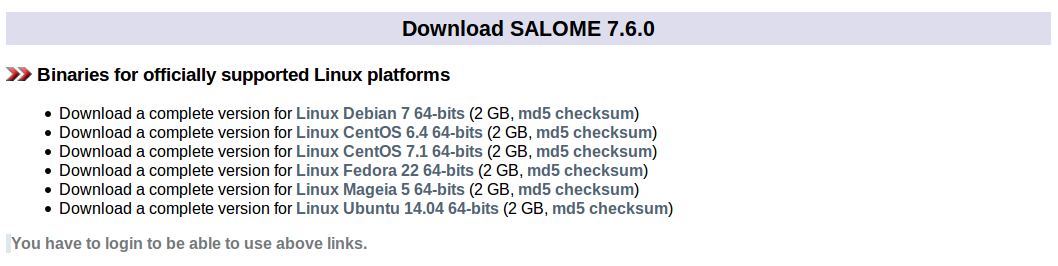
\includegraphics[scale=0.35]{\LocCHtwelvefig/mesh_12_1.png}
\caption{Meshed geometry in Salome working window}
\label{mesh_1}
\end{figure}   

\section{Creating Groups}

In Mesh we can create a group of elements of a certain type. This helps us to identify the boundary patches in OpenFOAM. To create group from the top menu bar click on "Mesh" and slect "Create Group" To create a group once needs to define the following, \newline
\begin{itemize}
\item Mesh - The mesh from which elements will be selected to form the group. We can select the mesh in the Object Inspector Menu or in the 3D viewer.
\item Element type - These are a set of radio buttons which allows us to select the type of element which will form the group.
\begin{itemize}
\item Nodes
\item 0D elements
\item Ball
\item Edges
\item Faces
\item Volumes
\end{itemize}
\item Name - this field allows you to enter the name of the new group eg, "inlet"
\item Color - assigns color to a certain group. This helps to display the elements of a group
\item We can also distinguish between three group type as Standalone geometry, Group on geometry and group on filter.
\end{itemize}
 
\section{Grouping Mesh}
Since we have three patches in our geometry we will select the "Face" option from create groups and Group on geometry as the group type, this is because we will be grouping the elements of a certain type generated on our geometry. The Group on Geometry can be created only if the mesh is based on geometry. To define a group we choose the Group on geometry check box and then click the selection button besides Gemetrical object as shown in the figure \ref{mesh_1}. 

\begin{figure}[h]  
\centering
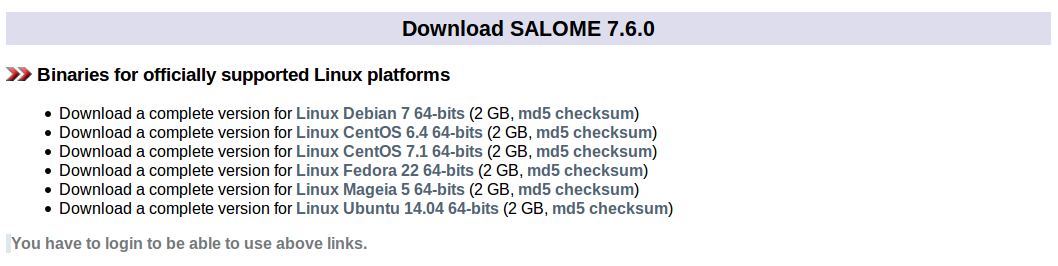
\includegraphics[scale=0.35]{\LocCHtwelvefig/mesh_12_1.png}
\caption{Meshed geometry in Salome working window}
\label{mesh_1}
\end{figure} 

Here we get two options
\begin{itemize}
\item Direct geometry selection - to select a shape in the Object Browser 
\item Find geometry by mesh element selection - to activate a dialog which retrives a shape by the selected element generated on this shape.
\end{itemize} //

We will use direct geometry selection since we have already grouped our geometry while creating the geometry. Open the geometry tree in the object browser and click on the Pipe$\_$1 and select the group which we had created during geometry such as "inlet", "outlet" and "walls". These faces can be identified by color by selecting a color from Color group . We can give names to this group of our choice , in this chapter we have kept the same name as that given in geometry i.e. "Inlet".Finally click on Apply and close to end the geometry selection. Follow the similar procedure for naming outlet faces of the mesh. Inlet and Outlet group will be seen in the Mesh-1 tree. For selecting the faces for walls we select the element type in Create group as Face and Group type as Group on Filter. Now we click on the set filter.This open a new box named as Filter for faces \ref{mesh_1}, click on the "Add" button. In the drop down menu below Criterion select "Free faces" and click on Apply and close. You can provide any color of your choice here. Click on Apply and close to create Group-1. From the menu bar now click on Mesh menu and select Cut of groups and select the main object as Group-1 as shown in figure \ref{mesh_1}. Click on tool object and from grouped object select Inlet, hold the shift key and select Outlet. We can see the Result name on top of the window, type "walls". Select any color of your choice and click on Apply and close. This will now create a group named "walls" in the Mesh tress in object browser. Delete the Group-1 in the mesh tree as we no longer need the group. We can save our work by clicking on the Save Document option just above object browser. To export the mesh file right click on Mesh-1 and select Export and click on UNV file. Name this file as "bentpipe" and save it in your working directory. Now we can close salome.

\section{Creating Case directory}

To solve this problem in OpenFOAM we need to first create a case directory in OpenFOAM. We will be using icoFoam solver to solver this problem, which is an incompressible transient solver for laminar flows. We create a directory inside icoFoam and name it as bentpipe. Copy the bentpipe.unv file which we had saved and paste this into the bentpipe folder. Now Copy the 0 and system folder from the cavity folder to the bentpipe folder. The directory structure of the bentpipe folder is as shown in the figure, \ref{mesh_1}.

\begin{figure}[h]  
\centering
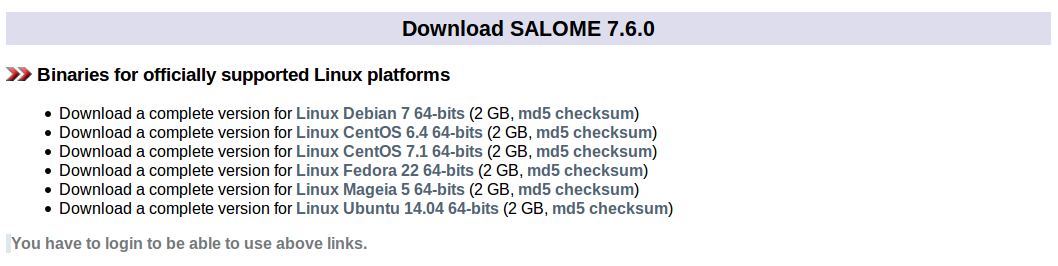
\includegraphics[scale=0.35]{\LocCHtwelvefig/mesh_12_1.png}
\caption{Meshed geometry in Salome working window}
\label{mesh_1}
\end{figure}

Note that, we have not copied the constant folder here as it will be created once we have converted our mesh file from UNV to Foam format. Open the terminal window and type the path for bentpipe inside the icoFoam solver as follows \\
/OpenFOAM/OpenFOAM-2.x.x/tutorial/incompressible/icoFoam/bentpipe \\

\subsection{Geometry conversion}

To convert the geometry from UNV format to OpenFOAM recognisable format we use the command as shown below, \\

ideasUnVToFoam -filename \\

The file name in our case would be bentpipe.unv. Once the file is converted we can see that the constant folder is created. The polyMesh folder inside constant folder stores the information regarding geometry, check this folder for files such boundary, faces, neighbours, owner, points. Also do not forget to copy the transportProperties file from the cavity folder and paste this inside the constant folder

\subsection{Geometry Scaling}     

In Salome, by default the geometry is created in millimeters. To convert the geometry from millimeters to centimeters we will use the OpenFOAM utility of transformPoints. In In the command terminal type  the command given below for using this utility and press enter\\

transformPoints -scale '(0.01 0.01 0.01)' \\

We will see that the geometry has been converted to centimeters.

\section{Setting 0 folder}

As we had copied the 0 folder from the cavity case we need to make changes inside the pressure (p) and Velocity (U) file for matching the boudnary names given in Salome. Open each file and insert the boundary name and boundary condition as shown in the table below for both pressure and velocity.


\section{Visualization}

The case directory tress for the bentpipe case will be as shown below, \ref{mesh_1}.

\begin{figure}[h]  
\centering
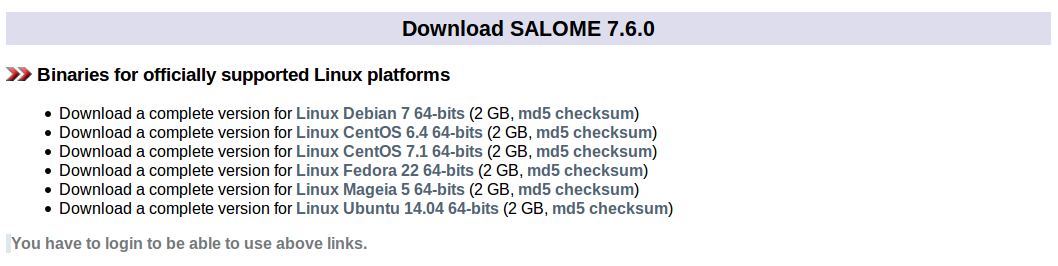
\includegraphics[scale=0.35]{\LocCHtwelvefig/mesh_12_1.png}
\caption{Meshed geometry in Salome working window}
\label{mesh_1}
\end{figure}

To visualize the geometry we will open Paraview using the paraFoam command in terminal.Click on Apply button in the Object Inspector menu, we will see the geometry as seen in the figure \ref{mesh_1}.

\begin{figure}[h]  
\centering
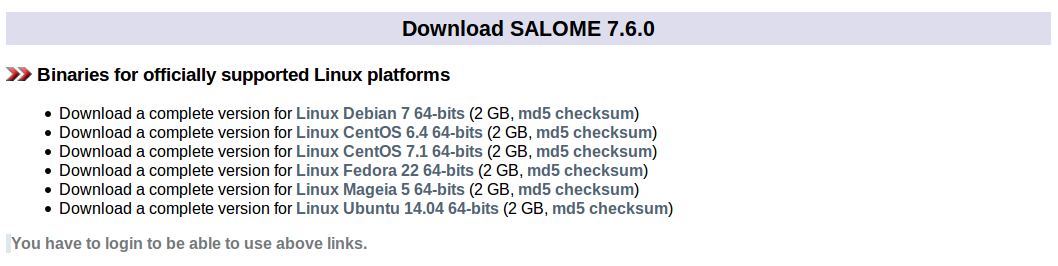
\includegraphics[scale=0.35]{\LocCHtwelvefig/mesh_12_1.png}
\caption{Meshed geometry in Salome working window}
\label{mesh_1}
\end{figure}

Now to view the mesh , from the drop down menu select Surface with Edges. Zoom into the geometry to see the mesh. In Mesh parts inside Object Inspector we can see that the groups have been properly created and match with that created in Salome namely "Inlet", "Outlet" and "Walls". Volume of pipe by default is named as "internalMesh". This bring us to the end of this chapter.

\section{Assignment}

In this chapter and the earlir chapter 11, we have seen how to create geometry, mesh the geometry and create groups for the mesh file to be imported inside OpenFOAM. As an assignment create a bentpipe with radius 5 mm and total length of 300 mm and export the geometry in "unv" file format. Finally visualize the results in OpenFOAM.


\chapter{Introduction to snappyHexMesh}
\thispagestyle{empty}
\label{sec:chap13}
\newcommand{\LocCHonethreefig}{\Origin/CHAPTERS/chap13/figures}

\section{What is snappyHexMesh}

The snappyHexMesh is a utility in OpenFOAM which a generates 3-dimensional meshes containing hexahedra (hex) and split-hexahedra (split-hex) automatically from triangulated surface geometries in Stereolithography (STL) format. The mesh approximately conforms to the surface by iteratively refining a starting mesh and morphing the resulting split-hex mesh to the surface. An optional phase will shrink back the resulting mesh and insert cell layers. The specification of mesh refinement level is very flexible and the surface handling is robust with a pre-specified final mesh quality. It runs in parallel with a load balancing step every iteration.\newline

\flushleft The basic requirements for generating a mesh using snappyHexMesh are as follows,

\begin{itemize}
\item STL File : The geometry stl file should be of good quality because it will be the reference surface for the snapping process. Expecially if there are curved surfaces, they will be jagged following the trace of stl file. If they are provided specific thickening to a particular surface of geometry, is recommended to define specific patch in stl file, this patch can be recognized and imported in snappyHexMeshDict file. The stl must be in constant/triSurface directory, in ASCII format
\item blockMesh : After stl creation is necessary to create the reference hexaedra mesh with blockMesh utility. This will be the "raw piece of rock" modelled by the sculptor (snappyHexMesh in this case) following the geometry described in stl files. The dimension of these blocks is the reference dimension (corresponding to 0 levels of refinement), starting from this it is possible to calculate the minimum cell size. The block can contain the whole stl surface, or you may decide to make it smaller in order to cut the geometry, it depends also on the type of mesh, internal or external.
The blockMeshDict file must be in constant/polyMesh directory and the blockMesh process can be started by typing blockMesh in the main folder of the case. It creates all mesh files (boundary, owner, points, ecc ecc) in constant/polyMesh directory.
snappyHexMesh is designed to work properly on base elements with unitary aspect ratio, despite this it is possible to operate on slightly stretched cells.

\end{itemize} 


\chapter{Generating mesh using SnappyHexMesh}
\thispagestyle{empty}
\label{sec:chap14}
\newcommand{\LocCHonefourfig}{\Origin/CHAPTERS/chap14/figures}


\chapter{Importing Mesh From Third Party Software in OpenFOAM}
\thispagestyle{empty}
\label{sec:chap15}
\newcommand{\LocCHonefivefig}{\Origin/CHAPTERS/chap15/figures}

OpenFOAM can be used for creating and meshing geometrical shapes like Box, Pipe. When dealing with complex geometries like a turbine blade, aircraft,
ship etc, we cannot use the blockMesh utility. In such cases it is always better to create the geometry and mesh in dedicated CAD and Meshing softwares 
and solve those usiing OpenFOAM. As a prerequisite it is expected the user should have knowledge about creating geometry and generating mesh in softwares
like Gmabit, Gmsh, Salome, ICEM etc. This chapter deals with the steps involved in importing mesh files in OpenFOAM using different mesh conversion tools.

\section{Geometry}

We will use the above problem of Flow over a square cylinder as an example for importing mesh file in OpenFOAM. Here we have a square cylinder
of length 1m and height 1 m. Inlet velocity is set at 1 $\frac{m}{s}$ for Reynolds number (Re) 100. The size of the domain choosen is 60 m by 40 m.
The boundary conditions are as shown in the , Fig \ref{square} below.

\begin{figure}[t]  
\centering  
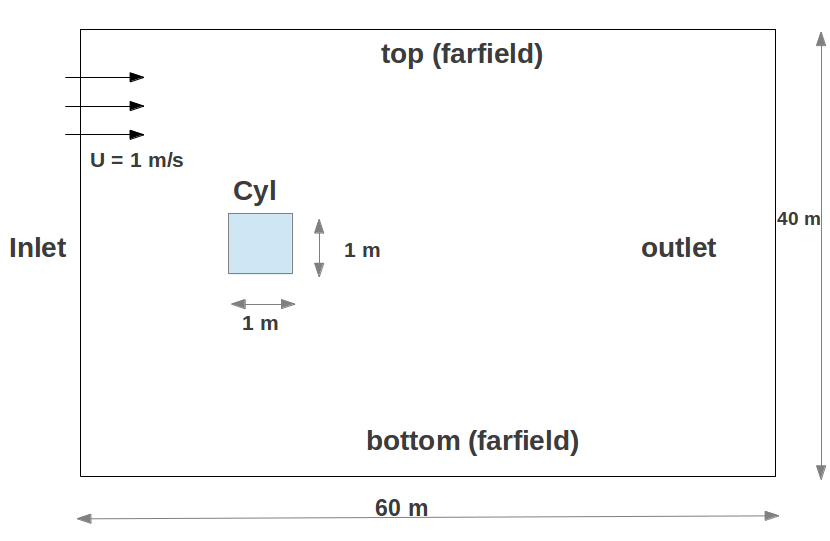
\includegraphics[width=\lgfig]{\LocCHonefivefig/square.png}
\caption{Flow over square Cylinder}
\label{square}  
\end{figure}

\section{Meshing}

We have generated a hexhedral mesh for the above geometry with 40000 cells and saved the mesh file as cylmesh.msh. 
The mesh generated is as shown below, Fig \ref{mesh} 

\begin{figure}[h]  
\centering
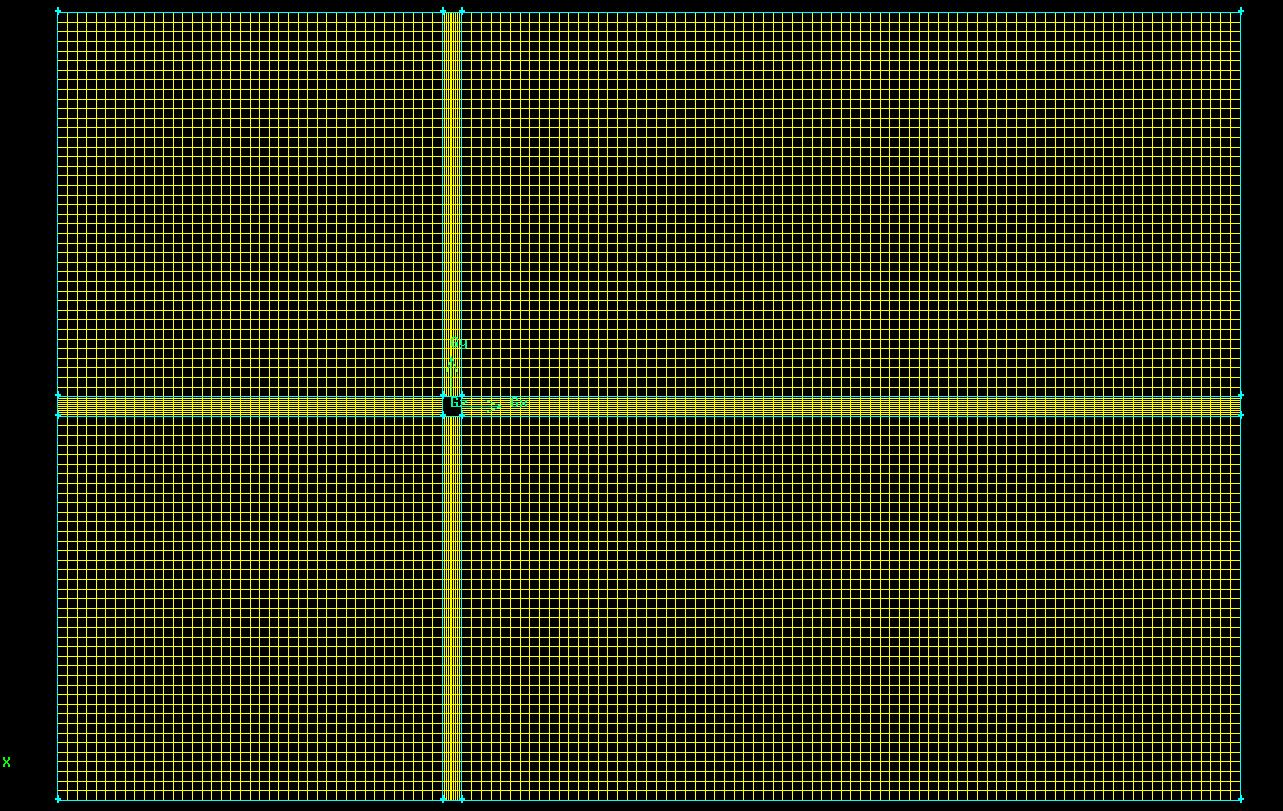
\includegraphics[width=\lgfig]{\LocCHonefivefig/cylmesh.jpeg}
\caption{Mesh}
\label{mesh}
  
\end{figure}

\section{Importing the mesh file}

In incompressibel solvers go to icoFoam and create a solver inside it by the name \textbf{cylinder}. Now go inside the cavity case and copy the 
\begin{itemize}
\item 0
\item system
\end{itemize}

\flushleft folder and paste it inside the cylinder folder. Please make a not here that we do not need the \textbf{constant} folder here. After this copy the 
cylmesh.msh mesh file create earlier and paste this inside this folder. Thus the our case file is now ready. Now open the command terminal and type the
path for the cylinder folder. Now since we have a Fluent (.msh) mesh file we will use the mesh conversion command as shown below followed by the file name \\
\centering \textbf{fluentMeshToFoam file-name.msh} \newline

\flushleft In the terminal window type the above command with the file name and press enter.

\begin{figure}[h]  
\centering
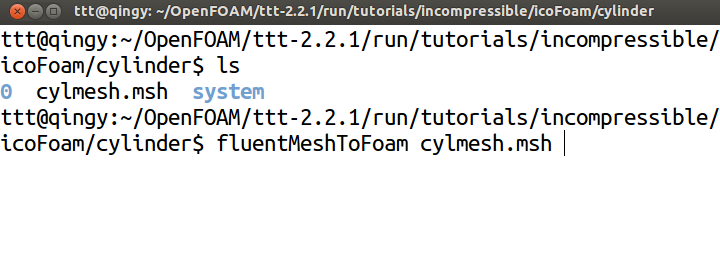
\includegraphics[width=\lgfig]{\LocCHonefivefig/conversion.png}
\caption{convert}
\label{mesh}
\end{figure}

\flushleft In case you have a 3D mesh file then you can use the command \\ \vspace{0.5cm}
\centering {\textbf{fluent3DMeshToFoam file-name.msh}} \newline

\flushleft The Fluent mesh file is converted into OpenFOAM mesh file. Now if we look back into our cylinder folder we can see that the "constant"
folder is now generated. When we open the constant folder we will see that the transport properties file is missing. Since we had converted the 
fluent mesh file into openfoam the fluid property files were missing. Copy the transport property file from the constant folder of cavity case
and paste this inside the constant folder of cylinder. The trasnportProperties file contains the value of fluid viscosity, we can either change it
or keep it default. \newline

\flushleft Make a note here that we do not use the \textbf{blockMesh} command here

\section{Boundary Conditions}

When we import the geometry in OpenFOAM we need to be very careful with the boudnary names used while creating the mesh file. Since OpenFOAM is case
sensitive in case of any mistake with the boundary names can create an error while running the solver. To view the boundary names in the command terminal
go to polyMesh folder inside the constant. Inside polyMesh you can see a file by the name \textbf{boundary}. Open this file in any editor of your
choice, eg, gedit boundary, Fig \ref{boundary}.

\begin{figure}[h]  
\centering
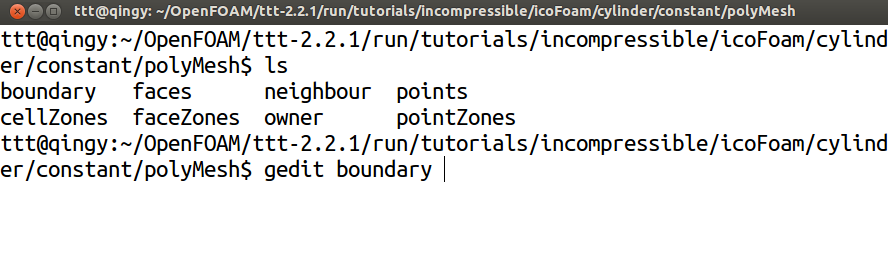
\includegraphics[width=\lgfig]{\LocCHonefivefig/boundary.png}
\caption{Boundary file}
\label{boundary}
\end{figure}

\flushleft The boundary names will be as shown in the domain shown above, Fig \ref{square}. In case of any error with the boundary names you can
always refer to this boundary file. Now in your command terminal go to the 0 folder and open the pressure file. Make sure that the boundary names 
match exactly the names in the boundary file, in case of errors make the necessary changes.

\section{Solver settings}

In the terminal window go to the controlDict file inside system and open it in any editor of your choice. Change the endTime from 0.5 to 1.5 seconds.
Save the file and close it, Fig \ref{cd} and come back to the cylinder folder.

\begin{figure}[h]  
\centering
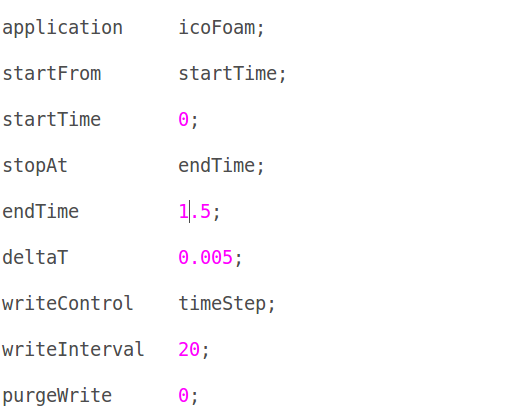
\includegraphics[width=\lgfig]{\LocCHonefivefig/controldict.png}
\caption{controlDict file}
\label{cd}
\end{figure}

\flushleft After making the necessary changes we can now run the solver. In the temrinal window type the name of the solver \textbf{icoFoam}
and press enter. The iterations will be seen running on the terminal window. After the iterations stop we can now start with the visualization.

\section{Post-Processing}

Launch paraview by typing \textbf{paraFoam} in the terminal window and once it opens click on the Apply button to view the geometry, Fig \ref{geom}.
In the active varialble control menu change from Solid Color to Velocity (U). You can now see the initial conditions for velocity, Fig \ref{vel}.
To view the animation on the right hand top of paraview click on the play button of VCR menu. You can see the change in velocity in the paraview 
window with the passage of time, Fig \ref {vel-1}.

\begin{figure}[h]  
\centering
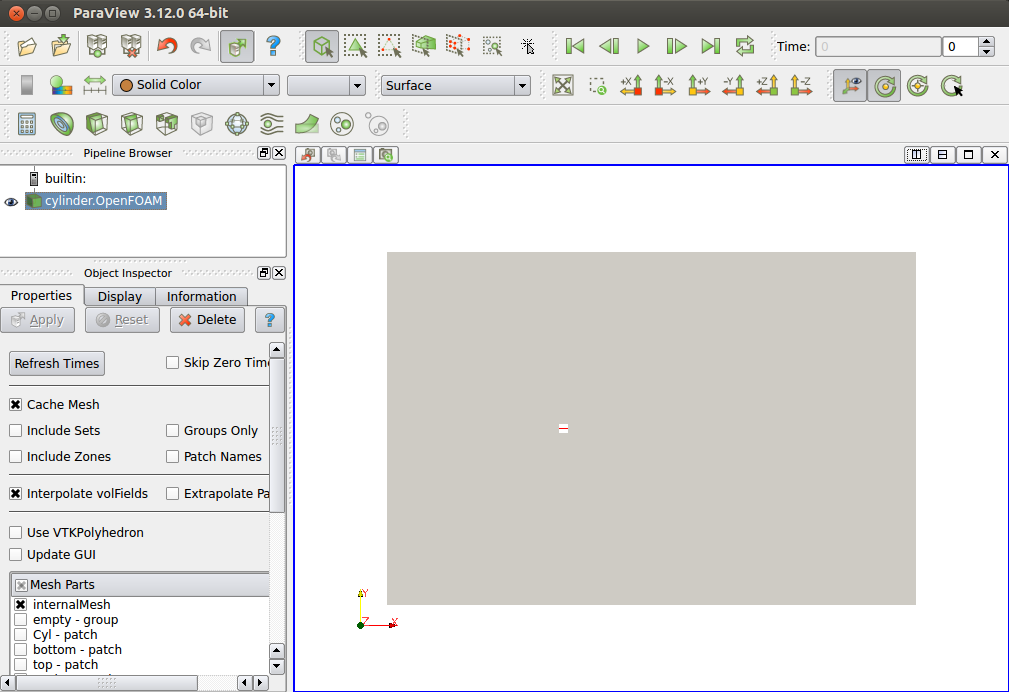
\includegraphics[width=\lgfig]{\LocCHonefivefig/geom-paraview.png}
\caption{Geometry in Paraview}
\label{geom}
\end{figure}

\begin{figure}[h]  
\centering
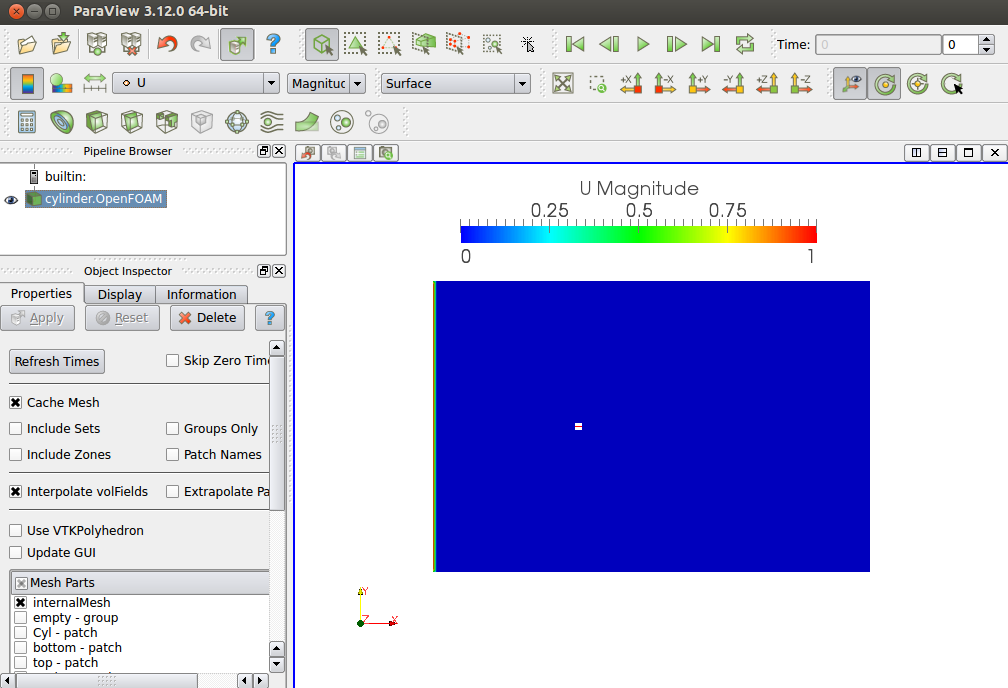
\includegraphics[width=\lgfig]{\LocCHonefivefig/vel.png}
\caption{Initial velocity condition}
\label{vel}
\end{figure}

\begin{figure}[h]  
\centering
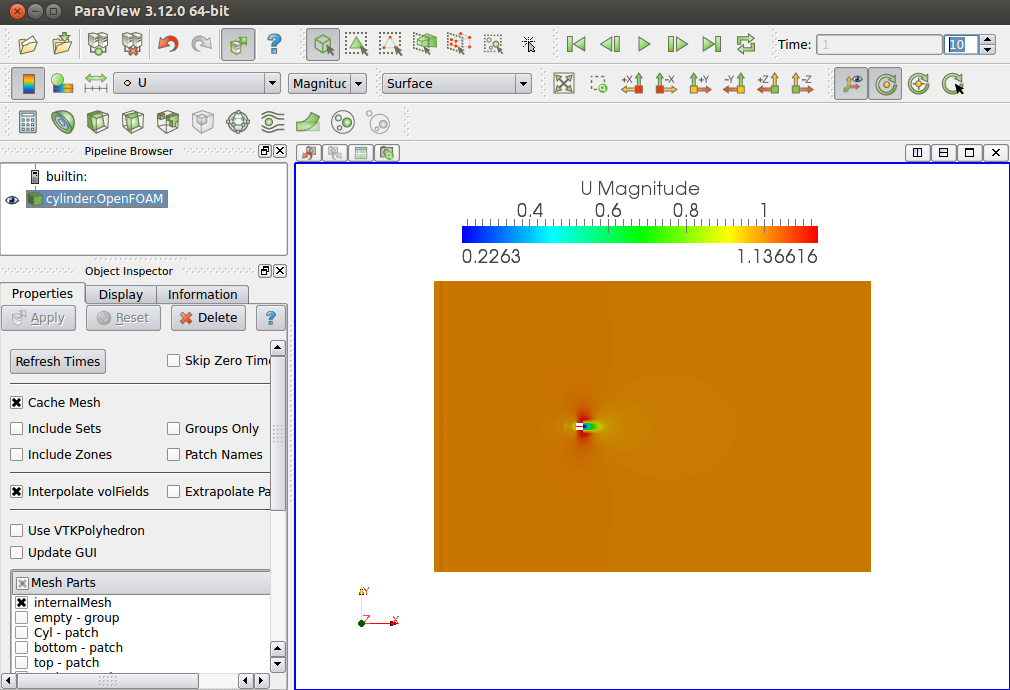
\includegraphics[width=\lgfig]{\LocCHonefivefig/vel-1.png}
\caption{Velocity at 1 sec}
\label{vel-1}
\end{figure}

\section{Mesh Conversion Commands}

The user can also import mesh files from other meshing softwares as well. Here is a list of commands to import mesh files in OpenFOAM.

\begin{itemize}
\item ANSYS : ansysToFoam file-name
\item IDEAS : ideasToFoam file-name
\item CFX : cfxToFoam file-name
\item SALOME : ideasUnvToFoam file-name
\end{itemize}


 %rahul
\chapter{Installing and Running Gmsh}
\thispagestyle{empty}
\label{sec:chap16}
\newcommand{\LocCHonesixfig}{\Origin/CHAPTERS/chap16/figures}

Gmsh is a Free and Open Source three dimensional finite element grid generator with a build-in CAD engine and post-
processor. There are four modules available in Gmsh such as Geometry, Meshing, Solver and Post-Processiing. The specification 
of any input to these modules is done either interactively using the graphical user interface or in ASCII text files using its own scripting language.
With Gmsh we can create and mesh a geometry and import it in OpenFOAM or import a CAD file (stl, step) and use it for OpenFOAM using the mesh conversion utilities (see chapter 17 for more info).
In this chapter we will cover how to install Gmsh and create a simple geometry.It is expected that the user should have knowledge 
about Meshing.

\section{Installing Gmsh}

Gmsh can be installed using Synaptic Package Manager. Open Gmsh in your system by typing your system password.
In the search box type Gmsh and install it, Fig \ref{synaptic-gmsh}. This might take some time depending on your internet speed.

\begin{figure}[ht]  
\begin{center}  
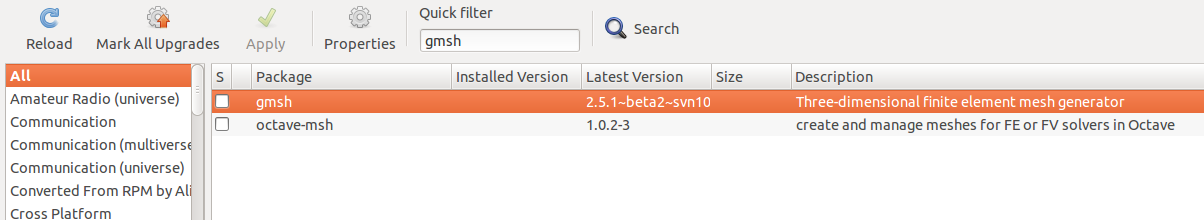
\includegraphics[scale=0.32]{\LocCHonesixfig/synaptic-gmsh.png}
\caption{Install Gmsh}
\label{synaptic-gmsh}
\end{center}  
\end{figure}


\flushleft Alternately we can also install Gmsh from the gmsh website given below,

\center {\textbf{http://geuz.org/gmsh/}} \newline

\flushleft Open this website in your browser and scroll down to download. Now Download Gmsh according to the given current stable release 
Fig \ref{download-gmsh} according to your Operating System (OS).

\begin{figure}[ht]  
\begin{center}  
\includegraphics[scale=0.352]{\LocCHonesixfig/download-gmsh.png}
\caption{Download stable release}
\label{download-gmsh}
\end{center}  
\end{figure}

\begin{figure}[ht]  
\begin{center}  
\includegraphics[scale=0.26]{\LocCHonesixfig/gmsh-icon.png}
\caption{gmsh-icon}
\label{gmsh-icon}
\end{center}  
\end{figure}

\section{Running Gmsh}

\flushleft In the Download folder extract the downloaded gmsh tar file. After you open the folder you will see folder named bin, click on it. 
Inide the bin folder you will see the Gmsh icon, Fig \ref{gmsh-icon}. Double click on it to launch the Gmsh Start screen, Fig \ref{gmsh-start} \newline

As a pracice to learn Gmsh we will create a cube of sides 1 unit as seen in the Fig, \ref{geometry1}. On the left hand side in the Gmsh window you can 
see three modules namely,

\begin{itemize}
\item Geometry
\item Mesh
\item Solver
\end{itemize}

Click on the Geometry module, then go to Elementary Entities, inside elementary entities go to add and then click on points. This will open up a
window where you can enter the X, Y and Z co-ordinates starting with 0 inside each box and press Enter, Fig \ref{point}. Now
enter points for all the remaining 7 vertices to complete the cube, Fig \ref{geometry1}. In the Gmsh screen we can see the eight points, you can move those points
using the left mouse click. To join these points click on Straight-line option under Elementary Entities. Now select any two points to create a straight line, click 
on the start point and then the second point to create a line. Similarly join all the other points to create a cube as shown in the Fig, \ref{line} below.
As you can see on the Gmsh screen you can press e to end selection and q to abort.

\begin{figure}[t]  
\begin{center}  
\includegraphics[scale=0.28]{\LocCHonesixfig/gmsh-start.png}
\caption{Gmsh Start window}
\label{gmsh-start}
\end{center}  
\end{figure}

\begin{figure}[t]  
\begin{center}  
\includegraphics[scale=0.28]{\LocCHonesixfig/geometry1.png}
\caption{Geometry for Gmsh}
\label{geometry1}
\end{center}  
\end{figure}

\begin{figure}[t]  
\begin{center}  
\includegraphics[scale=0.28]{\LocCHonesixfig/point-gmsh.png}
\caption{Points window}
\label{point}
\end{center}  
\end{figure}

\begin{figure}[t]  
\begin{center}  
\includegraphics[scale=0.28]{\LocCHonesixfig/cube-gmsh.png}
\caption{Join points using line}
\label{line}
\end{center}  
\end{figure}

\subsection{Create Faces}

To create faces for the cube click on plane-surface unde elementery enetities. After this select the outer booundaries of the face of a rectangle.
Select the edges of the bottom face first.Once you select the edges they will turn red in color, Fig \ref{face}. Check in case if there is any hole in the 
face, if none then press e to end selection. You will notice that a face will appear with dasshed center lines, Fig \ref{cl}. Repeat this procedure for 
remaining faces, Fig \ref{face-all} and finally press q to abort.

\begin{figure}[t]  
\begin{center}  
\includegraphics[scale=0.28]{\LocCHonesixfig/face-red.png}
\caption{Selct edges}
\label{face}
\end{center}  
\end{figure}


\begin{figure}[t]  
\begin{center}  
\includegraphics[scale=0.28]{\LocCHonesixfig/face-cl.png}
\caption{Bottom Face}
\label{cl}
\end{center}  
\end{figure}

\begin{figure}[t]  
\begin{center}  
\includegraphics[scale=0.28]{\LocCHonesixfig/face-all.png}
\caption{Create faces for all surfaces}
\label{face-all}
\end{center}  
\end{figure}

\subsection{Creating Volume}

We now need to create volume boundary. We need to select the Volume boundary similar to selecting boundary for faces. 
Click on the Volume boundary under elementery entities and click on boundary surface of the cube and press e to end selection. A yellow dot will
appear at the center of the cube which represents volume in Gmsh. Press q to abort the selction.

\begin{figure}[t]  
\begin{center}  
\includegraphics[scale=0.28]{\LocCHonesixfig/vol-gmsh.png}
\caption{Volume}
\label{vol}
\end{center}  
\end{figure}

\subsection{Physical Groups}

Physical groups heps us to identify a set of points, lines, faces, volume with a unique Identification number. We create physical groups which will be useful for exporting the Mesh file to OpenFOAM.To do so click on Physical Group under Geometry Module. Click on Add and then Surface. Upon selection of any face it will turn red. Now press e to end selection. Do this procedure for all the remaining facesand press q to abort. Also we need to select the Physical Volume. Click on Volume under Physical Groups and select the yellow dot at the center of the cube.The yellow dot will turn red in colour adn press e to end selection and q to abort.

To save the geometry under the file menu click on Save as and save the geometry by the name cube.geo. Here "geo" stands for geometry. Click OK twice
to save the geometry. 
 %rahul
\chapter{Creating a Sphere using Gmsh}
\thispagestyle{empty}
\label{sec:chap17}
\newcommand{\LocCHonesevenfig}{\Origin/CHAPTERS/chap17/figures}

In the earlier chapter we learnt about how to Install and Run Gmsh by creating a simple geometry. As the earlier tutorial shows about basic geometry construction in Gmsh the user is expected to know it before starting this chapter. This chapter deals with creating a Sphere using Gmsh and meshing it. The chapter we will focus on creating the spherical geometry and the domain surrounding it and in the next chapter we will look into how to mesh this geometry. Since this is a spherical geometry we will learn about how to create a circular arc, how to create ruled surface and doing basic manipulation with the .geo file which generated. 

\section{Points}

You can start Gmsh by either double clicking on the gmsh-icon or from the terminal by typing \textbf{gmsh sphere1.geo} , this will open up the gmsh window. The first step after starting Gmsh is to mark the co-ordinates for our sphere, we define the center of the Sphere and points surrounding it. Co-ordinates for the sphere ( 7 points ) are as given below : \newline

\begin{itemize}

\item (0, 0, 0)
\item (-1, 0, 0)
\item (1, 0, 0)
\item (0, -1, 0)
\item (0, 1, 0)
\item (0, 0, -1)
\item (0, 0, 1)

\end{itemize}

\flushleft The points will appear on the Gmsh window as shown in the Fig \ref{points} below.

\begin{figure}[h]  
\centering
\includegraphics[scale=0.25]{\LocCHonesevenfig/gmshpts.png}
\caption{Sphere coordinates}
\label{points}
\end{figure}

\section{Circular Arc}

Creating an Arc is a three step process where we a start point, center and an end point . An important point to be noted here is that in Gmsh a Circular Arc is strictly created less than pi. Now to create an circular arc select Circle Arc option in the left hand side menu of Gmsh under Add. Click on the right most point in the Gmsh Window, it will turn red in colour, Fig \ref {point1}.

\begin{figure}[h]  
\centering
\includegraphics[scale=0.25]{\LocCHonesevenfig/point1.png}
\caption{Rightmost point}
\label{point1}
\end{figure}

\flushleft Now click on the center of the Sphere as shown in Fig \ref{point2} and that too will turn red in colour.

\begin{figure}[h]  
\centering
\includegraphics[scale=0.25]{\LocCHonesevenfig/point2.png}
\caption{Center of the sphere}
\label{point2}
\end{figure}

\flushleft For the end point click on the point above the center. As soon as we click on this point a arc is created as shown in the Fig \ref{point3}.

\begin{figure}[h]  
\centering
\includegraphics[scale=0.25]{\LocCHonesevenfig/point3.png}
\caption{End point of the Arc}
\label{point3}
\end{figure}

\flushleft Repeat this process for all the points to complete the sphere. Create the Arcs keeping the same center point. The completed geometry of the sphere is as shown , Fig \ref{}

\begin{figure}[h]  
\centering
\includegraphics[scale=0.25]{\LocCHonesevenfig/sphere.png}
\caption{Sphere}
\label{sphere}
\end{figure}

\section{Surface Creation}

To stich the arcs together we now need to create surfaces. To do so, click on the Ruled Surface option under Add menu. Now select bounding edges for the surface as shown in Fig \ref{surface}. After the selction they will turn red in colour. Press e on your keyboard to execute this selection. A crossed dotted line will be visible which shows that the surface has been created, Fig \ref{surf1}. Repeat the process to create all eight surfaces of the sphere, Fig \ref{surf2}.

\begin{figure}[h]  
\centering
\includegraphics[scale=0.25]{\LocCHonesevenfig/surface.png}
\caption{Surface Bounding edges}
\label{surface}
\end{figure}

\begin{figure}[h]  
\centering
\includegraphics[scale=0.25]{\LocCHonesevenfig/surf1.png}
\caption{Surface Creation}
\label{surf1}
\end{figure}

\begin{figure}[h]  
\centering
\includegraphics[scale=0.25]{\LocCHonesevenfig/surf2.png}
\caption{Complete Surface Creation}
\label{surf2}
\end{figure}

\section{Editing .geo file}

Gmsh provides us with an option of editing the saved file. Open sphere1.geo file in any editor of your choice. Information related to the geometric entities we create using Gmsh are stored here. General syntax under gmsh is as given below,\newline

\centering Point (1) = {0,0,0,1}; \newline

\flushleft here Point stand for the Geometrical Entity, (1) stands for Identification number inside the parenthesis next number starting from one which is equal to an expression. For points in expression we have the X, Y and Z co-ordinate followed by the value of desired mesh element size. The size of the mesh element will then be computed by linearly interpolating these values on initial mesh. We can change the mesh element size here by a variable which can then take different value. Change the mesh element size from 1 to s and on top of the file type s = 0.1; as shown in the Fig \ref{var}

\begin{figure}[h]  
\centering
\includegraphics[scale=0.35]{\LocCHonesevenfig/var.png}
\caption{Mesh Element size variable}
\label{var}
\end{figure}

\section{Boundary Layer}

Flow over any bluff body we are more interested in capturing the Boundary Layer. In this problem to capture the boundary layer in the geo file add a line after the mesh characteristic length varialble as \newline

\centering  \textbf{Mesh.CharacteristicLengthFromCurvature = 0.05;} \\

\flushleft This line above will adapt the mesh to the curvature w.r.t the geometrical entities.

\section{Volume Creation}

To create a volume we need all the bounding surfaces. This can also be done manually by typing at the end of the file \newline

\centering \textbf{Surface Loop (identity) = {identities of sphere surface within braces};} \\

\flushleft Now save this file and close it

\section{Physical Groups}

The geometry created now needs a physical meaning to it which helps us during simulation. To do this under Physical Groups go to Surface and select all the 8 surfaces of the sphere. It will turn red in colour, Fig \ref{surf4}. Press e to end selction and q to abort. Now again open the sphere1.geo file. It can be noticed that a new line has been added to the file which describes the physical surface. Here replace the Identification number by the name sphere within double quotes as this can be used as a boundary identification during simulation or postprocessing.\newline

\centering \textbf{Physical Surface("Sphere") = {26, 27, 28, 30, 31, 32, 33, 34};} \\

\flushleft Save and close the file. 

\begin{figure}[h]  
\centering
\includegraphics[scale=0.25]{\LocCHonesevenfig/surf4.png}
\caption{Physical Groups : Surface}
\label{surf4}
\end{figure}
 


 %rahul
\chapter{Unstructured mesh Generation using Gmsh}
\thispagestyle{empty}
\label{sec:chap18}
\newcommand{\LocCHoneeightfig}{\Origin/CHAPTERS/chap18/figures}

In the previous chapter we saw how to create a Sphere in Gmsh. This chapter is a continuation of the last chapter and it is expected that the user has practiced and gone through it. Gmsh being a finite element mesh generator can be used to generate unstructured mesh (tri, prisims, etc). Since mesh generation is an important step in CFD simulation, we will look into the steps required to generate unstructured meshes and also make some changes in the geometry (.geo) file of Gmsh.

\section{Geometry}

Flow over a sphere has a vast engineering application. These simulations provide a test of the ability of the code to accurately reproduce typical flow structures observed in generic bluff body flows, such as those experienced by submarines and Unmanned Underwater Vehicles (UUVs). The geometry setup for our case is as shown in the Fig \ref{geom} below. We can see that the right left side of the geometry is termed as Inlet and the right side is termed as outlet which shows that the flow will move from left to right. The remaining sides of the geometry such as the top, bottom and side wslls are kept as empty. Sphere is fixed at the center of the domain. Length of the domain is 45 x 45 x 30 (L x B x H ) and radius of the sphere is 1 (Chapter 17). We have used this as an example in this chapter and actual dimensions can vary from case to case.
    
\begin{figure}[h]  
\centering
\includegraphics[scale=0.35]{\LocCHoneeightfig/geom.png}
\caption{Geometry for mesh generation}
\label{geom}
\end{figure}
    
\section{Creating Domain}

We need to create domain around the sphere as seen in the Fig \ref{geom}. Use the Geometry module in Gmsh to generate points (Chapter 16). Since it is a 3 Dimensional geometry we have eight points in our domain as given below,

\begin{itemize}
  \item (-15 ,-15 ,-15)
  \item (-15 , 15 ,-15)
  \item (-15 ,-15 , 15)
  \item (-15 , 15 , 15)
  \item ( 30 ,-15 ,-15)
  \item ( 30 , 15 ,-15)
  \item ( 30 ,-15 , 15)
  \item ( 30 , 15 , 15)
\end{itemize}

\flushleft Join all these points using lines (Straight Line) option under points. The final geometry will be as shown in Fig \ref{final-geom}.

\begin{figure}[h]  
\centering
\includegraphics[scale=0.35]{\LocCHoneeightfig/final.png}
\caption{Creating and joining points}
\label{final-geom}
\end{figure}

\section{Surface and Volume}

We will now create surface for the geometry. Note that in this case we are using the option Plane surface instead of Ruled Surface. The difference between the two is that Ruled surface is used for creating a surface that can be interpolated using transfinite interpolation i.e. Sphere and a Plane Surface can be used for creating a planar surface. Now select four edges of a face, as we had seen in the previous chapter these edges turn red in Color upon selection, Fig \ref{surf}. After we select the four edges press e to end selection and q to abort. Repeat this process for the remaining faces. Once the a surface is created you notice a dotted crossed line, Fig \ref{surf1}.

\begin{figure}[h]  
\centering
\includegraphics[scale=0.35]{\LocCHoneeightfig/surf.png}
\caption{Surface Selection}
\label{surf}
\end{figure}

\begin{figure}[h]  
\centering
\includegraphics[scale=0.35]{\LocCHoneeightfig/surf1.png}
\caption{Surface Creation}
\label{surf1}
\end{figure}

\subsection{Physical Groups}

The purpose of physical entities is to assemble elementary entities into larger, possibly overlapping groups, and to control the orientation of the elements in these groups.
Since we require boundary names in our mesh file we group the faces under one commom name.\\

\flushleft Go to Physical Surface > Add > Surface and select a surface according to the boundary names given in the Geometry setup. Select the left face first since it is the Inlet, Fig \ref {inlet} and press e to end selection. Now click on the right face for outlet, Fig \ref{out} and press e to end selection. The remaining sides of the geometry are walls, so select all the four sides, Fig \ref{wall} and press e to end selection.

\begin{figure}[h]  
\centering
\includegraphics[scale=0.35]{\LocCHoneeightfig/inlet.png}
\caption{Physical Groups : Inlet}
\label{inlet}
\end{figure}

\begin{figure}[h]  
\centering
\includegraphics[scale=0.35]{\LocCHoneeightfig/out.png}
\caption{Physical Groups : Outlet}
\label{out}
\end{figure}

\begin{figure}[h]  
\centering
\includegraphics[scale=0.35]{\LocCHoneeightfig/walls.png}
\caption{Physical Groups : Walls}
\label{wall}
\end{figure}

\flushleft Since we are working on the same geometry file (Sphere1.geo) we will now open this file in a text editor. Note that there are new points added here. Also the Identification number for the entities are in continuation of the earlier series eg, In the .geo file on top we can see Points along with its Identification number 7. Now the new Point created has an Identification Number 8. As we had seen in the earlier chapter we can change the mesh element size, change the last variable in Points from 1 to d as shown below for all the points from 8 to 15 and at the beginning of the file type d = 0.5 and end it with a semi-colon.

\begin{itemize}
  \item Point(8) = {-15, -15, -15, d};
\end{itemize}

\flushleft Now we need to name the Physical Surfaces we created earlier. We need to replace the Identification number for the Surface under Physical Surfaces (54) to desired name of our boundary as shown below. It is important to keep in mind the order in which we selected the faces here, since that will be the boudnary name for that particular face when we export the file in OpenFOAM. As we had selected the first face as the left face we will name it as Inlet.

\begin{itemize}
  \item Physical Surface ("Inlet") = {51};
\end{itemize}

Replace the Identification number by the Boundary name "Inlet", do not forget to use these double quotes. Repeat this for Outlet and Walls.

\subsection{Volume}

To define the Volume we need to build surfaces, for this one has to define surface loops. In the .geo file now at the bottom of the file type,

\begin{itemize}
  \item Surface Loop() = {};
\end{itemize}

\flushleft In round brackets Identification number is the next integer after the Identification number in Physical Surface, In my case it is 63. In the currly brackets enter the ID's of the Plane Surface, in our case we have 6 faces and hence 6 ID's. The Surface Loop will be as shown below,

\begin{itemize}
  \item Surface Loop(63) = {49, 51, 53, 55, 57, 59};
\end{itemize}

\flushleft After we define the Surface Loop we can now create Volume for th mesh. Type this line after the Surface Loop as shown below,

\begin{itemize}
  \item Volume() = {};
\end{itemize}

\flushleft Inside the round brackets enter 64 as the next Identification number after 63 in Surface Loop. Since we have two volumes in our geometry i.e Sphere and the Rectangular domain we will enter the respective Surface Loop ID's here as shown below.

\begin{itemize}
  \item Volume(64) = {36, 63};
\end{itemize}

Finally we need to create a Physical Volume. To do this in the next line under Volume type the Line given below,

\begin{itemize}
  \item Physical Volume()={};
\end{itemize} 

\flushleft Under round brackets enter 65 as the next Identification number after 64 in Volume. On the right hand side under curely brackets enter the Identification Number for Volume i.e 64. Our file is now ready, we can save it and close.

\begin{itemize}
  \item Physical Volume(65)={64};
\end{itemize}

\section{Meshing}

Now in Gmsh open the geometry file (Sphere1.geo) that we just saved. Gmsh follows a bottom to top approach for meshing i.e first we start with 1D meshing for meshing the edges of the geometry. Followed by 2D meshing for surfaces and Finally 3D Meshing for Volume. You can either mesh the geometry using the Mesh module in Gmsh or using F1 key for 1D meshing, F2 for 2D meshing and F3 key for 3D Meshing. We will now select F1 key for 1D meshing, we can see the message in the console below stating that 1D meshing is done, Fig \ref(1d). Now press F2 key for 2D meshing, Fig \ref{2d} and Finally press F3 key for 3D mehsing, Fig\ref{3d}.

\begin{figure}[h]  
\centering
\includegraphics[scale=0.35]{\LocCHoneeightfig/1d.png}
\caption{One Dimensional Meshing}
\label{wall}
\end{figure}

\begin{figure}[h]  
\centering
\includegraphics[scale=0.35]{\LocCHoneeightfig/2d.png}
\caption{Two Dimensional Meshing - Surface }
\label{wall}
\end{figure}


\begin{figure}[h]  
\centering
\includegraphics[scale=0.35]{\LocCHoneeightfig/3d.png}
\caption{Three Dimensional Meshing - Volume}
\label{wall}
\end{figure}

\flushleft We can also optimize the mesh using the Optimize funtions available under the mesh module. Click on the Optimize 3D netgen option.
 %rahul
%\input{user-code/sw-env/sw-env.tex}
%\input{user-code/led/led.tex}
%\input{user-code/push/push.tex}
%\input{user-code/ldr/ldr.tex}
%\input{user-code/dcmotor/dcmotor.tex}
%\input{user-code/pot/pot.tex}
%\input{user-code/servo/servo.tex}
%\input{texfiles/servo.tex}
%\input{texfiles/Appendix.tex}
%\appendix
%\input{texfiles/sp-appendix.tex}
%\input{windows/windows}

%\bibliography{bibliography.bib}
%\printindex
%\input{texfiles/AuthorInfo.tex}
\end{document}
